\documentclass[12pt]{article}

% ---- geometry: exactly 1 inch on all four sides ----
\usepackage[letterpaper,top=1in,bottom=1in,left=1in,right=1in]{geometry}

% ---- maths first, then a Times New Roman equivalent (newtx wants this order) ----
\usepackage{amsmath}
\usepackage{amssymb}
\usepackage[T1]{fontenc}
\usepackage{newtxtext}
\usepackage{newtxmath}

\usepackage{graphicx}
\usepackage{array}
\usepackage{longtable}
\usepackage[table]{xcolor}
\definecolor{tblhead}{gray}{0.85}
\usepackage{adjustbox}
\usepackage{changepage}                 % adjustwidth for the abstract
\usepackage[font=small,labelfont=bf,labelsep=colon,justification=justified,
            skip=6pt]{caption}
\usepackage{titlesec}
\usepackage{ragged2e}
\usepackage{csquotes}
\usepackage{cite}                        % numeric [1], [2,3], compressed [4-6]
\usepackage[hidelinks]{hyperref}

% ---- body text: 12 pt, justified, 0.2 in first-line indent ----
\setlength{\parindent}{0.2in}
\setlength{\parskip}{3pt}
\linespread{1.10}
\setlength{\emergencystretch}{2em}   % avoid under/overfull boxes cheaply

% ---- decimal section headings: "N Title" (no period), up to 3 levels ----
\titleformat{\section}{\normalfont\Large\bfseries}{\thesection}{0.7em}{}
\titlespacing*{\section}{0pt}{16pt}{8pt}
\titleformat{\subsection}{\normalfont\large\bfseries\itshape}{\thesubsection}{0.7em}{}
\titlespacing*{\subsection}{0pt}{12pt}{6pt}
\titleformat{\subsubsection}{\normalfont\normalsize\bfseries\itshape}{\thesubsubsection}{0.7em}{}
\titlespacing*{\subsubsection}{0pt}{10pt}{4pt}
% titlesec suppresses the first-line indent right after a heading by default

\captionsetup[table]{position=below}

\newcommand{\abstitle}[1]{\noindent{\large\bfseries #1}\par\vspace{8pt}}

\pagestyle{plain}
\begin{document}
\thispagestyle{plain}

\begin{center}
{\LARGE\bfseries SafeNodule-MAS: A Reproducible, Cost-Aware, and\\[3pt]
Safety-Calibrated Multi-Agent Architecture for Lung Nodule Diagnosis\par}
\vspace{16pt}
{\large
Lochan Narayan K\textsuperscript{1}\quad Manikandan R\textsuperscript{1,*}\par}
\vspace{6pt}
{\small\itshape
\textsuperscript{1}School of Computing, SASTRA Deemed University, Thanjavur, Tamil Nadu, India\\
\upshape\texttt{lochannarayan11@gmail.com}\qquad\texttt{manikandan75@core.sastra.edu}\\
\upshape\textsuperscript{*}Corresponding author\par}
\vspace{16pt}
\end{center}

\abstitle{Abstract}
\begin{adjustwidth}{0.25in}{0.25in}
{\normalsize\selectfont\justifying Multiagent systems built from large language models are increasingly proposed for clinical decision support, yet published designs rarely make their orchestration, evidence grounding, uncertainty handling, or cost measurable. This paper presents an enhanced architecture for lung nodule diagnosis that keeps a published pipeline of 3 stages, detection, report generation, and malignancy reasoning, and adds 7 mechanisms, each with a measurable outcome, not an accuracy claim: an adaptive triage router, a role specific specialist board with weighted voting, a report grounded evidence verifier, a devil's advocate agent that guards against missed cancer, guideline grounded escalation to Lung RADS categories, temperature scaling fitted by likelihood on a held out split, and a margin based abstention gate. The system is evaluated on a reproducible synthetic harness under 5 stress regimes, 64 cases per seed across 8 seeds, and reporting accuracy, macro F1, coverage, false negative rate, calibration error, verifier precision and recall, and mean model calls per case, each with 95% confidence intervals and paired bootstrap significance tests. The specialist board raises accuracy in 4 of 5 regimes, though under a benign heavy prior a single unbiased agent performs better, a finding the framework reports. Adaptive routing cuts model calls per case by 2 to 4\%, and the text volume those calls carry by up to 7\%, a direct proxy for inference energy and price. The verifier flags every fabricated citation with high precision, and fitted calibration corrects most distribution shift error without disturbing already calibrated cases. The abstention gate helps only where confidence is informative, motivating a structural safeguard for the remaining cases. SafeNodule-MAS also advances sustainable healthcare computing by reducing computational redundancy through adaptive, multiagent orchestration. Overall, this work offers a reproducible blueprint in which safety, cost, and efficiency are measured properties of a multiagent diagnostic system, not assumed ones.\par}
\end{adjustwidth}
\vspace{8pt}
\noindent{\normalsize\selectfont\textbf{Keywords:} Multiagent systems; Clinical decision support; Selective prediction; Confidence calibration; Sustainable computing.\par}
\vspace{18pt}
\section{Introduction}

Lung cancer is the leading cause of cancer death worldwide, with an estimated 1.8 million deaths in 2022 [1]. Low-dose computed tomography (CT) screening reduces lung-cancer mortality in high-risk populations [2], and the pulmonary nodules it surfaces are the earliest actionable signal of disease. Turning a screen-detected nodule into a management decision requires three tasks in sequence: localizing the nodule on the volume, describing its morphology in clinically meaningful terms, and grading its malignancy risk with appropriate hedging. Radiologists perform these tasks by inspecting many slices per scan, which is time-consuming and subject to interobserver variability, and they anchor the final judgement in structured criteria such as the Fleischner Society recommendations [3], Lung-RADS [4], and quantitative risk models [5].


The operational burden is substantial. A screening CT contains hundreds of axial sections; a single scan can show several nodules, the large majority of which are benign, and each must be localized, measured, characterized, and assigned a follow-up interval. Because most findings are not cancer, the cost of the workflow is dominated by the surveillance it generates rather than by the cancers it catches, and small differences in how a nodule is measured or how a margin is judged propagate into different Lung-RADS categories and different recommendations. Reader studies consistently find non-trivial interobserver variability in nodule detection, in diameter and volume measurement, and in categorical malignancy assessment, and that variability is itself a source of downstream cost and of missed or delayed diagnoses [3]. Structured reporting and quantitative decision aids reduce this variability, which is why any automated assistant is expected to produce not just a label but the measurements and the criterion-referenced reasoning that support it [4,5].


Automation of the three tasks has a long history, and each is now individually strong. What has not been solved is delivering the tasks as one trustworthy process. Task-specific deep networks report high aggregate metrics but expose only a score, not the features or the pattern behind it, and their behaviour under a shifted scanner, protocol, or population is hard to anticipate. Clinical adoption of software as a medical device is gated less on peak accuracy than on traceability, calibrated uncertainty, monitoring, and a defined human-in-the-loop; a system that cannot say why it answered, or how sure it is, or when it should defer, is difficult to validate and difficult to supervise once deployed. These are the properties this paper measures.


Deep learning has improved each task in isolation (detection and segmentation networks localize nodules accurately [6], and classifiers grade malignancy from cropped volumes), but task-specific models are opaque and brittle under distribution shift, and they do not produce the chain of evidence a clinician needs to accept or override a prediction. General-purpose vision-language models (VLMs) such as GPT-4 [7], the Claude~3 family [8], Qwen2.5-VL [9], and LLaVA [10] add fluent explanation and broad world knowledge, and medical VLMs (LLaVA-Med [11], MedGemma [12], Med-R1 [13]) narrow the domain gap. Yet VLMs remain weak at the fine-grained quantitative perception nodule assessment needs, they hallucinate findings that are not present in the image [14], and their verbalized confidence is poorly calibrated [15]. Large models can encode clinical knowledge [16] and answer medical questions well [17], but knowledge recall is not the same as a trustworthy, auditable diagnostic process [18].


Collaborative multi-agent systems are a natural response. Debate among role-playing agents improves factuality and reasoning [19,20], structured multi-agent evaluation improves consistency [21], and the pattern has been carried into software engineering [22] and into medicine: MedAgents [23], MDAgents [24], MedAgent-Pro [25], and MedRAX [26] all coordinate several LLM roles, often with retrieval or tool use. Yang et~al.~[27] instantiate this pattern for lung nodules as LungNoduleAgent: a Nodule Spotter that coordinates detection models through mixture-of-experts inference, intersection-over-union (IoU) mask clustering, and a judging panel; a Simulated Radiologist that produces a localized report from a focal crop [28]; and a Doctor Agent System in which reasoning agents, each backed by a medical knowledge graph [29], revise their opinions and iterate until consensus. On two private datasets and LIDC-IDRI [30] it outperforms strong VLM and medical-agent baselines.


Consensus, however, is not the property that determines whether such a system can be deployed. A clinical decision-support tool must decide \emph{how much} deliberation a case warrants, so that routine nodules do not incur the cost of a full multi-agent discussion while difficult ones receive more scrutiny; it must keep every claim in the final explanation traceable to the shared evidence, so that a reviewer can see which statements are observed, reported, or inferred; it must surface disagreement rather than dissolve it, because a confident wrong consensus is more dangerous than an acknowledged split; it must express \emph{calibrated} uncertainty and be permitted to abstain when the evidence is insufficient, rather than being prompted to \enquote{always be definitive}; and it must account for its own computational cost, which for a stack of language-model calls is the dominant driver of latency and price at deployment. None of these behaviours is quantified in the original work: the number of debate rounds, the stopping rule, the provenance of the knowledge base, the calibration of the output probabilities, and the per-case call count are all left unspecified. This matters beyond engineering tidiness: calibration [31,32], selective prediction [33], and evidence grounding [34] are exactly the properties a regulator or a clinical adopter will ask a vendor to demonstrate.


Consider each unmeasured behaviour in turn. \emph{Deliberation allocation}: running a four-role board with multiple revision rounds on every nodule, including the obviously benign ones, multiplies the language-model call count without a corresponding accuracy gain; a triage step that reserves the board for ambiguous morphology should recover most of that cost, but only if the easy cases can be identified reliably and the router rarely down-triages a hard case. \emph{Claim provenance}: the original agents cite morphological features to justify their grade, but nothing checks that a cited feature actually appears in the report the pipeline produced, so a hallucinated sign can drive a confident diagnosis undetected. \emph{Disagreement}: iterating \enquote{until consensus} rewards conformity, and a board that converges quickly on the wrong label is worse than one that reports an honest split; there is no agent whose role is to resist the emerging answer and to guard specifically against a missed cancer. \emph{Uncertainty}: the agents are prompted to be definitive, the output probabilities are never calibrated against outcomes, and the system cannot decline. \emph{Cost}: the per-case number of model calls -- the quantity that determines latency and price -- is never reported. Each of these is a concrete, testable gap, and each admits a small mechanism with a measurable endpoint.


This article describes SafeNodule-MAS (LungNoduleAgent-Enhanced), an implementation that keeps the detect--describe--diagnose pipeline and turns each of these behaviours into an instrumented component with an explicit success metric. We deliberately do not claim a higher headline accuracy (Yang et~al.~[27] already report up to 89.1\% on LIDC-IDRI) because the contribution is methodological: a design in which safety and cost are first-class, measurable properties, evaluated under controlled stress with confidence intervals and significance tests, including the regimes in which a mechanism fails. To make the evaluation fully reproducible and independent of proprietary models or restricted datasets, the entire pipeline runs against a deterministic mock language backend and a synthetic CT generator; every module is a documented interface with a drop-in point for a real detector, a real VLM, and real DICOM data.


Recent work in sustainable computing emphasizes energy-aware and resource-efficient artificial intelligence, particularly as large models are deployed at scale in clinical settings [35,36,37]. Training and serving large language models carries a documented energy and carbon cost [35], and healthcare imaging AI is no exception [36,37]. SafeNodule-MAS is designed with this constraint in view: the triage router and the Chair's early-convergence rule exist specifically to avoid running the full four-role board, and its multiple debate rounds, on cases that do not need them, so that computational cost, and by extension energy use, scales with case difficulty rather than with a fixed worst-case budget.


A synthetic harness is a deliberate methodological choice, not a shortcut. Studying safety mechanisms requires the ability to \emph{dial in} the failure modes they target (unsupported claims, borderline lesions, class imbalance, degraded perception) at known rates, which is not possible on a fixed clinical benchmark where those conditions occur at whatever frequency the data happen to contain and cannot be isolated. It also removes two confounds that dominate LLM evaluation: non-determinism, so that an ablation reflects the mechanism rather than sampling noise, and data governance, so that the full protocol can be released and re-run. The obvious cost is external validity: absolute accuracy on synthetic data is uninformative, and because the mock reasoner and the label generator share a feature model, inter-agent error correlation is understated. We therefore restrict our claims to the quantities that transfer (the \emph{direction} and \emph{significance} of each component's effect, the calibration and grounding behaviour, and the per-case cost), and we treat the protocol, not the numbers, as the contribution to be reused on real data.


\textbf{Scope.} This paper is not a new model: the reasoning backbone is a pluggable interface and the detector is a placeholder. It is not a clinical validation: no patient data are used and no clinical performance is claimed. It is an architecture-and-evaluation contribution: a set of small, testable safety and cost mechanisms bolted onto a published pipeline, plus a controlled protocol that shows, for each mechanism, whether and where it earns its place.


\textbf{Contributions.} (i)~An architecture that adds seven safety and cost mechanisms to a published multi-agent lung-nodule pipeline, each paired with a specific quantitative endpoint (Table~1) and expressed as a small, testable algorithm (Algorithms 1 and 2). (ii)~A five-regime synthetic stress protocol (clean, feature noise, borderline sampling, class imbalance, and an adversarial combination) that deliberately exercises the failure modes the mechanisms target, together with a perceived-versus-oracle split so that agents and the verifier reason from imperfect perception while scoring uses ground truth. (iii)~A multi-seed evaluation with 95\% intervals and paired bootstrap tests, reporting both positive and negative results: confidence-based abstention loses value under class imbalance and heavy distribution shift, and a benign-heavy prior makes the role-differentiated board underperform a single unbiased agent. (iv)~A fully deterministic, dataset-free reference implementation, experiment runner, and test suite. The remainder of the paper is organized as follows. Section~2 reviews nodule assessment, detection, medical VLMs and agents, calibration, and adaptive computation. Section~3 details the architecture, the algorithms, the stress regimes, and the metrics. Section~4 reports the five-regime results, the ablation, and the significance tests. Section~5 discusses safety as a measurable property, the conditions under which selective prediction fails, and the path to a clinical evaluation. Section~6 concludes.

\section{Background and Related Work}\label{sec:bg}
\subsection{Pulmonary nodule assessment and guidelines}

Nodule management is governed by structured criteria. The Fleischner Society recommendations key follow-up to nodule size and density (solid, part-solid, ground-glass), with part-solid nodules carrying the highest malignancy risk [3]. Lung-RADS assigns a screening category (2--4X) and a recommended action, and escalates for spiculation and for a growing solid component [4]. Quantitative models such as the Brock model predict malignancy probability from size, morphology, and clinical context [5]. A system that claims to be \enquote{evidence-based} should therefore ground its output in a named, versioned criterion rather than in an unspecified knowledge base; our guideline agent does this explicitly (Section~3.3). The criteria also encode a specific asymmetry: the categories that trigger tissue sampling exist because a missed invasive cancer is far more costly than an unnecessary short-interval follow-up. Any automated grader that aggregates several opinions inherits the responsibility to preserve that asymmetry, which motivates a guard aimed specifically at false negatives rather than at overall error. The malignancy targets in this work follow the three-way pre-invasive / minimally-invasive / invasive adenocarcinoma scheme used by Yang et~al.~[27], in which the two invasive classes are the clinically actionable ones.

\subsection{The LungNoduleAgent pipeline}

Yang et~al.~[27] decompose lung-nodule analysis into three modules. The \emph{Nodule Spotter} divides the CT volume into slices, runs a mixture of detection experts in parallel, reconciles their candidate masks by IoU-distance clustering with DBSCAN, and passes the survivors to a judging panel of vision-language models that vote each candidate up or down with a confidence weight; the accepted mask is then measured. The \emph{Simulated Radiologist} takes a focal crop of the slice and mask, preserving surrounding context, and generates a localized report with a medical prompt that fixes the output format and forbids speculative language. The \emph{Doctor Agent System} gives several reasoning agents access to a medical knowledge graph built from authoritative sources with a GraphRAG-style construction and community-summary retrieval [29]; each agent grades the nodule, a summarizer compiles the opinions, and the agents revise and re-discuss until they agree. A shared memory stores the images, measurements, reports, and conversation. The present work leaves the Spotter and the Radiologist essentially intact and concentrates on the orchestration and governance of the Doctor Agent System and on the boundaries around it.

\subsection{Nodule detection and mask consensus}

Detection and segmentation of small 3D structures is mature: self-configuring frameworks such as nnU-Net [6] provide strong baselines, and ensembles of detectors reduce false positives. LungNoduleAgent combines several detectors through mixture-of-experts inference and then reconciles their masks by clustering: the distance between two masks is $d(m_i,m_j)=1-\mathrm{IoU}(m_i,m_j)$, masks are grouped with DBSCAN [38], and a judging panel of VLMs votes each surviving candidate up or down with a confidence weight [27]. We reimplement this consensus mechanism exactly in NumPy so that it is transparent and seed-deterministic.

\subsection{Vision-language models in medicine}

General VLMs [7,8,9,10] generalize well but underperform on specialized imaging because their pretraining is dominated by natural images and they lack domain priors. Medical VLMs adapt them with domain data and reinforcement learning [11,12,13], and large proprietary models reach strong medical-QA scores [16,17]. Two limitations persist and motivate the present work: fine-grained quantitative perception (measuring a nodule, judging a margin) remains weaker than dedicated models, and both classes of model hallucinate (asserting findings absent from the image [14]), which is precisely what an evidence verifier must catch. A third, quieter limitation is that VLM confidence, whether taken from token probabilities or elicited in words, does not track correctness well [15,39]; a pipeline that surfaces a probability to a clinician therefore cannot rely on the raw model output and needs an explicit calibration stage. The region-level prompting used by LungNoduleAgent, adapted from describe-anything work for medical images [28], mitigates the perception gap by focusing the model on a masked crop with surrounding context, but it does not address grounding or calibration, which remain the responsibility of the downstream reasoning stage.

\subsection{Multi-agent LLM systems and debate}

Letting several LLM instances argue and revise improves factuality and reasoning [19], encourages divergent hypotheses [20], and yields more reliable evaluation [21]; the pattern scales to complex collaborative tasks [22]. In medicine, MedAgents [23] and MDAgents [24] coordinate specialist roles, MedAgent-Pro [25] adds an evidence-oriented workflow, and MedRAX [26] sequences multimodal inputs for chest radiography. Reported weaknesses in pulmonary applications are difficulty with mixed-density nodules, limited use of longitudinal information, and weak agreement with histopathology [27]. A recurring gap is that debate is run for a fixed or unspecified number of rounds and terminates on \enquote{consensus} without a defined convergence test, and without a counter-agent whose job is to resist premature agreement. Two further properties are usually left implicit. The aggregation rule is often an unweighted majority, which discards the fact that different roles carry different authority for different questions and that agents report different confidences; and the compute budget is fixed rather than matched to case difficulty, so an easy question and a hard one cost the same. Kim et~al.~[24] address the second point by adapting the collaboration structure to difficulty, which is the pattern our triage router follows. The design in this paper makes the convergence test, the aggregation weights, the counter-agent, and the difficulty-matched budget all explicit and, more importantly, measured.

\subsection{Calibration and selective prediction}

A probability is calibrated if, among predictions made with confidence $q$, a fraction $q$ are correct. Temperature scaling divides the logits by a single scalar $T$ fitted to minimize negative log-likelihood on a held-out set and is a strong post-hoc calibrator for modern networks [31]; expected calibration error (ECE) summarizes the gap between confidence and accuracy over bins [32]. Selective prediction lets a model abstain: it trades coverage for a lower error rate on the answered subset, and the risk--coverage curve characterizes the trade-off [33]. LLM confidence, whether read from token probabilities or elicited verbally, is often miscalibrated [15,39], so a multi-agent medical system that aggregates several such signals needs an explicit calibration and abstention stage, and an evaluation that reports when that stage helps and when it does not.

\subsection{Evidence grounding and hallucination detection}

Hallucination, content unsupported by the input, is the central reliability problem for generative models [14]. Self-consistency checks [34] and retrieval-grounded generation [29] reduce it. In an agentic diagnostic pipeline the natural anchor is the localized report: if a specialist cites a morphological feature, that feature should appear in the report the Simulated Radiologist produced. Our verifier operationalizes this by parsing the report into the set of asserted facts and grading each cited feature against it, deliberately grounding on the pipeline's own artefact rather than on a hidden oracle.

\subsection{Adaptive computation}

Routing easy inputs through a cheaper path and reserving expensive computation for hard ones is a standard efficiency lever; MDAgents [24] adapts the collaboration structure to question difficulty. For a lung-nodule pipeline the analogue is a triage step that sends unambiguous morphology (a small smooth ground-glass nodule, a large obviously spiculated mass) to a single specialist and one round, and reserves the four-role board and multi-round debate for ambiguous cases. The value of such a router is an empirical question (how many cases are confidently easy, and how often does the router mistakenly down-triage a hard case) that we answer directly.

\subsection{Evaluating medical AI beyond accuracy}

A recurring lesson from clinical machine learning is that a single aggregate accuracy figure is a poor predictor of deployed behaviour. Four additional axes matter here. First, \emph{calibration}: a model whose 0.9-confidence predictions are right only 70\% of the time will mislead a clinician who uses the probability as a decision threshold [31,32]. Second, \emph{selective risk}: the operating point of a system that can defer is a (coverage, risk) pair, and two systems with the same overall accuracy can differ sharply in how safely they behave when allowed to abstain [33]. Third, \emph{subgroup and prevalence robustness}: performance measured on a balanced benchmark can invert on a screening population where malignancy is rare, because thresholds and any class-dependent bias in the model interact with the base rate. Fourth, \emph{cost}: for an LLM pipeline the number and size of model calls set the latency, the price, and the carbon footprint, and a method that improves accuracy by an order of magnitude more compute is not obviously an improvement. Our evaluation reports all four axes alongside accuracy, and treats a component as justified only when it moves its designated axis in a pre-registered direction with a significant paired effect.

\section{System Architecture and Evaluation Protocol}\label{sec:method}

Figure~1 shows the resulting four-stage pipeline. Stage~1 (Nodule Spotter) and Stage~2 (Simulated Radiologist) are retained from Yang et~al.~[27], with the mixture-of-experts, IoU--DBSCAN clustering, and confidence-weighted judging panel reimplemented in NumPy. Stage~0 (Triage Router) and Stage~3 (Doctor Board) carry the new mechanisms detailed in this section: a role-differentiated board, a report-grounded evidence verifier, a Devil's-Advocate false-negative guard, a Chair with an explicit convergence test and debate loop, fitted temperature scaling with a margin abstention gate, and a Lung-RADS guideline agent, with hierarchical memory and a Medical Graph RAG store spanning all stages.


\begin{figure*}[htbp]
\centering
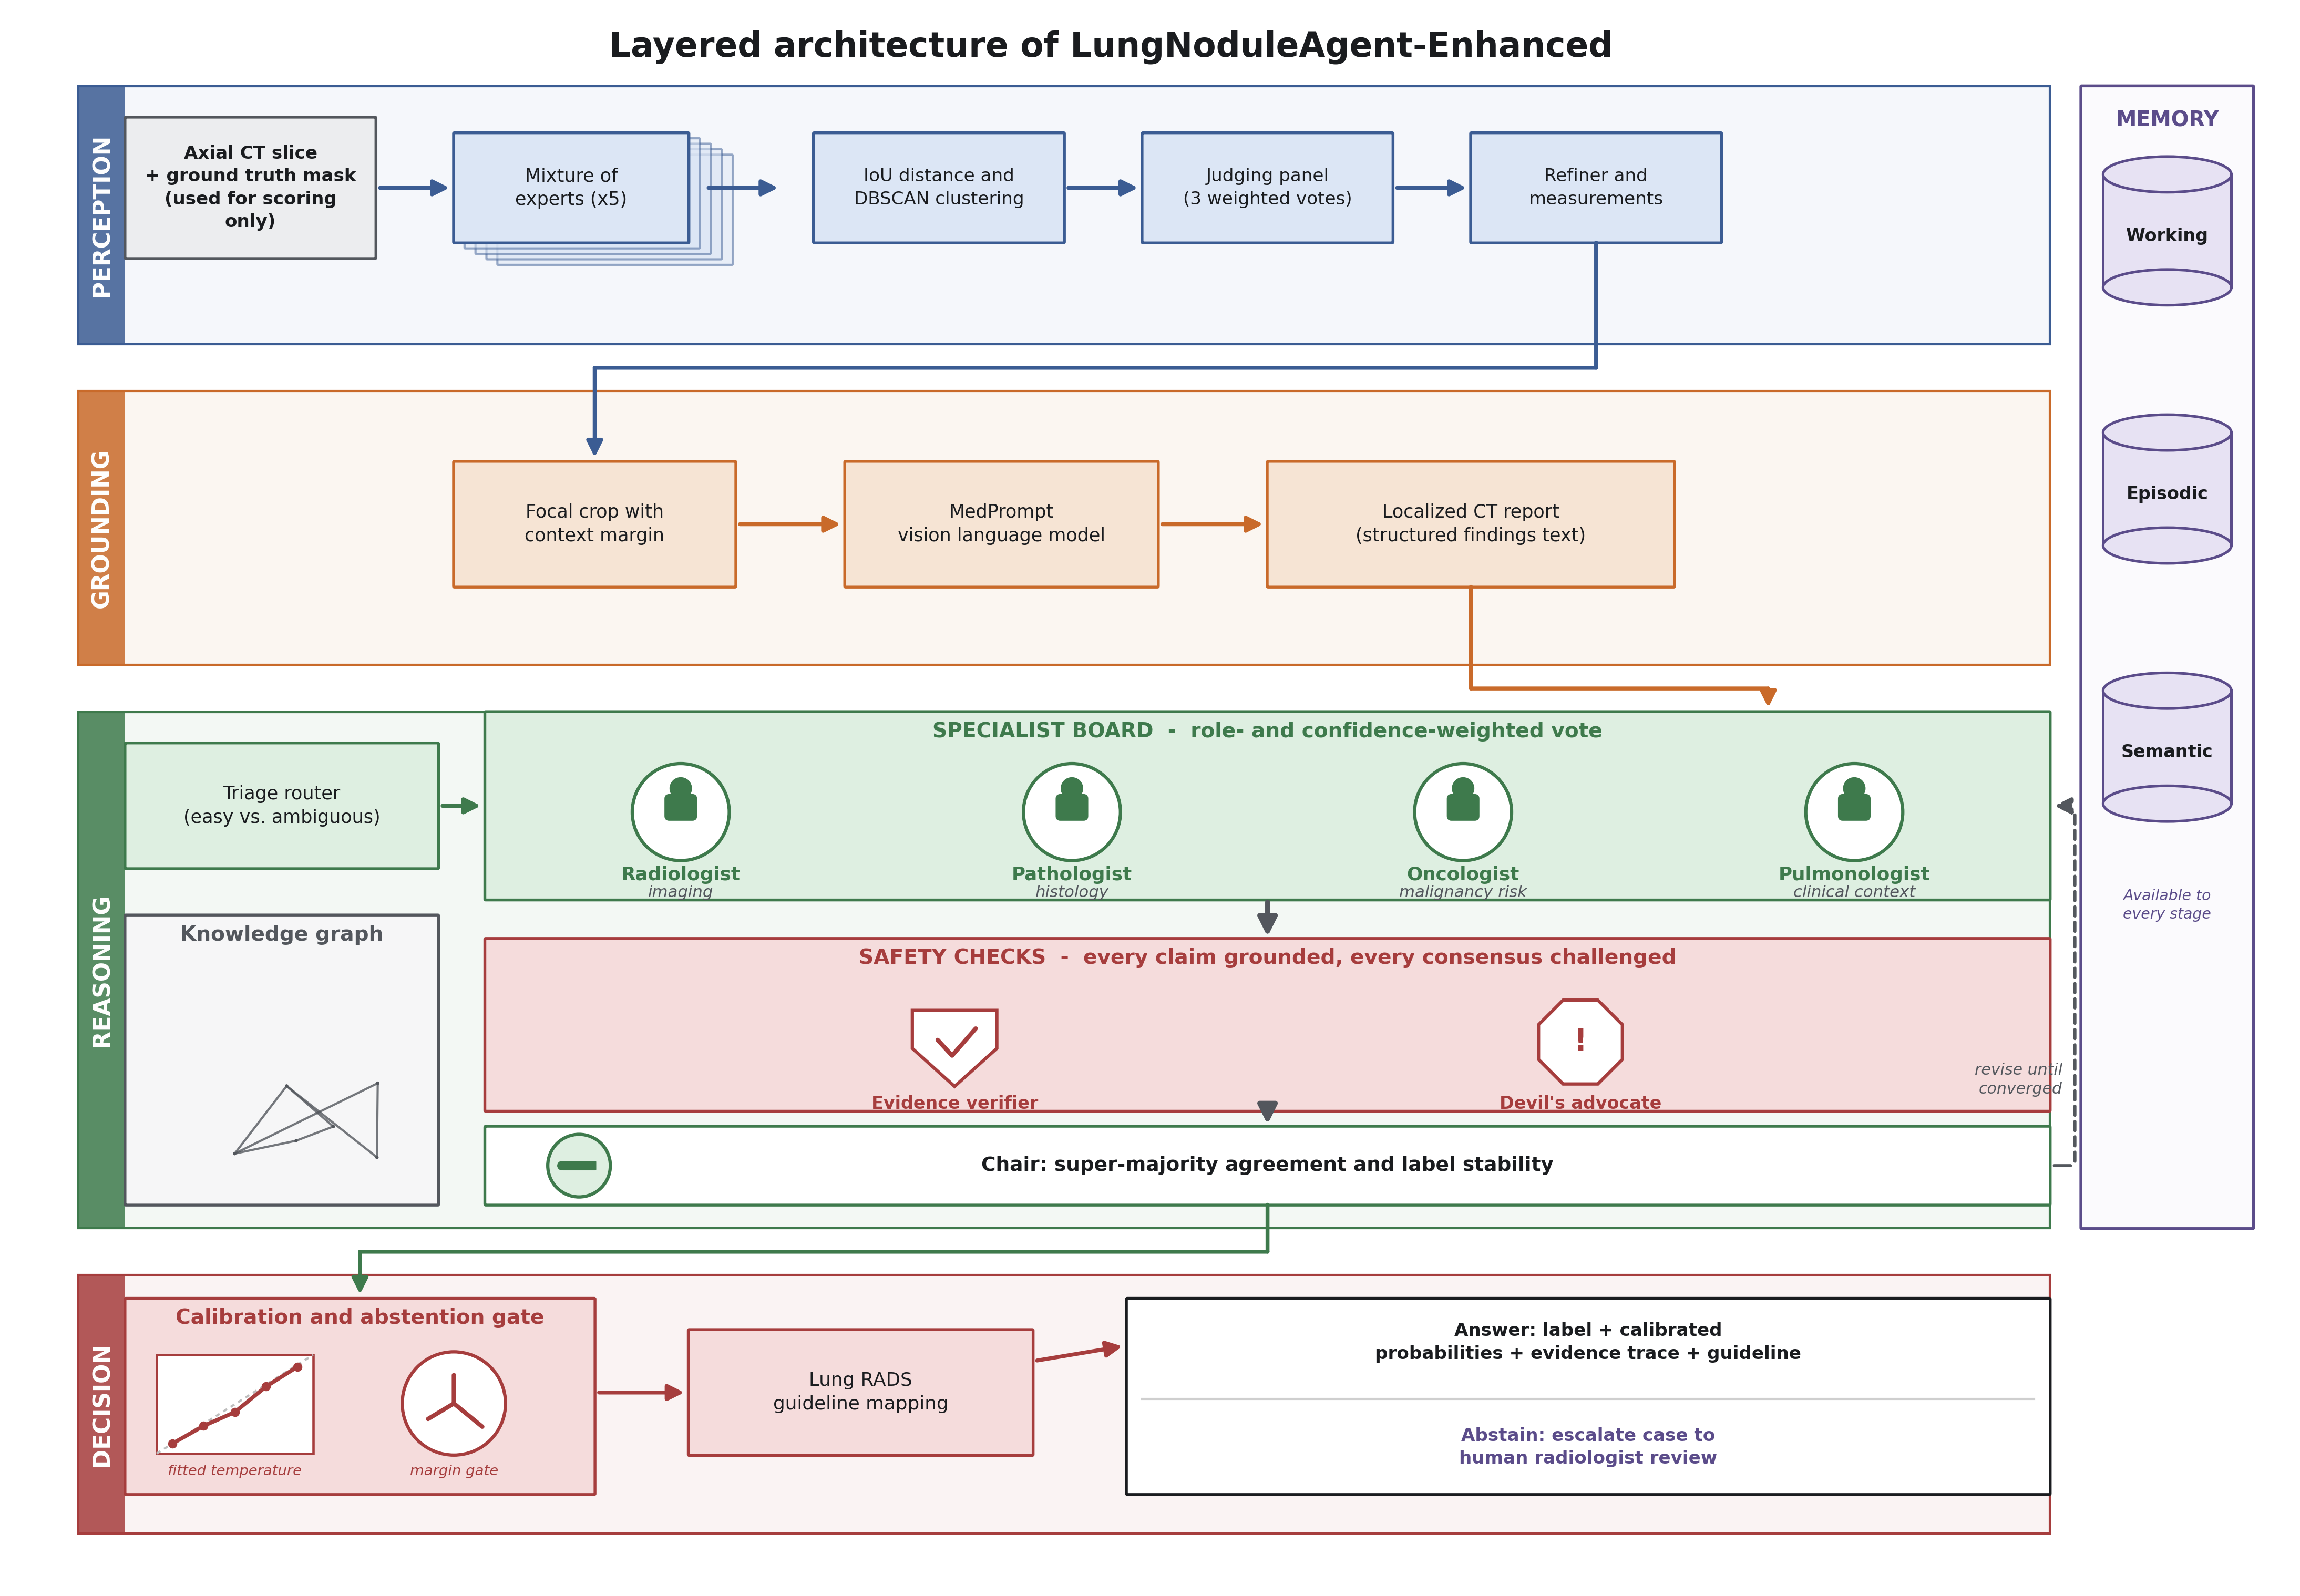
\includegraphics[width=0.98\textwidth]{figures/architecture.png}
\caption{LungNoduleAgent-Enhanced pipeline architecture.}
\label{fig:arch}
\end{figure*}

\subsection{Relationship to the original framework}

The enhancement is an extension, not a replacement. The Nodule Spotter still performs mixture-of-experts detection, IoU-distance DBSCAN mask clustering, and confidence-weighted judging-panel voting; the Simulated Radiologist still produces a localized report from a focal crop with a context margin; the Doctor Agent System still performs malignancy reasoning with retrieved knowledge and multi-round discussion. The new components sit inside and around the Doctor Agent System and at the pipeline boundaries, and every original interface is preserved so that the two designs can be compared component by component.

\subsection{An evidence taxonomy}

The design separates three kinds of evidence that agentic systems routinely conflate. \emph{Image-derived} evidence is the final mask and the measurements taken from it: long and short diameter and an estimated volume $V=\tfrac{1}{6}\,d_{\text{long}}\,d_{\text{short}}\,h$. \emph{Report-derived} evidence is the morphology the Simulated Radiologist asserts: lobar location, density, margin, shape, and the presence or absence of spiculation, pleural indentation, vascular convergence, air bronchogram, and cavitation. \emph{Knowledge-derived} evidence is the guideline and pathology text retrieved for each role. Keeping these distinct is what makes the verifier meaningful: a specialist's cited feature is checked against the report, not against a private oracle, so the verifier catches inconsistency introduced by the agent rather than error inherited from perception.

\subsection{Enhanced components and their success criteria}\label{sec:comp}

Table~1 pairs each enhanced component with the regime-wise metric used to judge it, rather than a single headline accuracy number, so that the endpoint decides whether the component earns its place.

\begin{table}[htbp]
\centering
\small
\renewcommand{\arraystretch}{1.25}
\setlength{\tabcolsep}{5pt}
\begin{adjustbox}{max width=\linewidth}
\begin{tabular}{|p{0.15\textwidth}|p{0.46\textwidth}|p{0.31\textwidth}|}
\hline
\rowcolor{tblhead}
\textbf{Component} & \textbf{Function} & \textbf{Success metric} \\ \hline
Triage router & easy $\to$ 1 specialist, 1 round; ambiguous $\to$ 4-role board, $\le$4 rounds; decision recorded with its reason & mean LLM calls/case; fraction routed easy; under-triage rate \\
\hline
Role-differentiated board & thoracic radiologist, pathologist, oncologist, pulmonologist; each queries a role-specific knowledge subgraph; role- and confidence-weighted aggregation & accuracy and macro-F1 vs.\ a single agent (paired test) \\
\hline
Evidence verifier & parses the report; grades each cited feature as supported, unmentioned (soft flag), or contradicted (hard flag); penalizes confidence by $0.05$/$0.20$ & hard-flag precision and recall vs.\ the oracle; flags/case \\
\hline
Devil's-Advocate & argues the strongest alternative each round; if the board leans benign while it puts $\ge 0.60$ on malignancy, escalate to human review & false-negative rate vs.\ the board without it (paired test) \\
\hline
Guideline agent & maps size and density to Lung-RADS v2022; spiculation, pleural indentation, and documented growth escalate the category & escalation correctness (deterministic unit tests) \\
\hline
Fitted calibration & temperature fitted by NLL on a 30\% held-out split of each run, then applied to the remainder & ECE at $T{=}1$ vs.\ fitted $T$; the fitted $T$ per regime \\
\hline
Abstention gate & abstain when the calibrated top-1/top-2 margin $<0.10$, when the top probability $<0.40$, or when the Devil's-Advocate guard fires & risk--coverage AURC; abstention value $=\mathrm{err}_{\mathrm{abst}}-\mathrm{err}_{\mathrm{ans}}$ \\
\hline
\end{tabular}
\end{adjustbox}
\caption{Enhanced components and their success metrics.}
\label{tab:components}
\end{table}


\textbf{Aggregation.} Each specialist $i$ returns a distribution $P_i$ over the three malignancy classes and a self-reported confidence $c_i$. The board aggregates with role weights $w_{\text{role}}$ (oncologist $1.2$, radiologist and pathologist $1.0$, pulmonologist $0.9$, Devil's-Advocate $0.6$): $\bar P(k)=\big(\sum_i c_i\,w_{r(i)}\,P_i(k)\big)/\sum_i c_i\,w_{r(i)}$. Temperature scaling then produces the calibrated distribution $\tilde P(k)\propto \exp\!\big(\log \bar P(k)/T\big)$, and the abstention gate reads its top-1/top-2 margin and entropy. \textbf{Verifier grading.} For a claim $x$ and the parsed report claims $C$: $x$ is \textsc{supported} if $C$ asserts it, \textsc{contradicted} if $C$ asserts its negation (a hard flag, $-0.20$ confidence), and \textsc{unmentioned} otherwise (a soft flag, $-0.05$). \textbf{Convergence.} The Chair stops the debate when a super-majority ($\ge 0.75$) of specialists share the leading label and that label is stable across two rounds, or at the round limit.

\subsection{Algorithms}

Algorithm~1 and Algorithm~2 state the debate loop and the calibration and abstention decision exactly as coded. Notation: $\mathcal{S}$ is the set of specialist roles, $P_i$ and $c_i$ the distribution and self-reported confidence returned by role $i$, $X_i$ the set of features that role cites, $w_{r(i)}$ its role weight, $\bar P$ the weighted aggregate, $\tilde P$ the calibrated aggregate, $\alpha_t$ the agreement at round $t$, $\ell_t$ the leading label at round $t$, and $E$ the evidence trace. The three classes are pre-invasive, minimally invasive, and invasive; the latter two are the malignant classes the guard protects.


Figure~2 traces the same two procedures as a flow: how the triage router splits the case, how the specialists, the Evidence Verifier, the Chair and the Devil's-Advocate interact inside one debate round, where the single feedback edge closes the loop, and in what order weighted aggregation, temperature scaling, the abstention gate and the false-negative guard apply before the review packet is emitted. Both triage paths share that calibration spine.


\begin{figure*}[htbp]
\centering
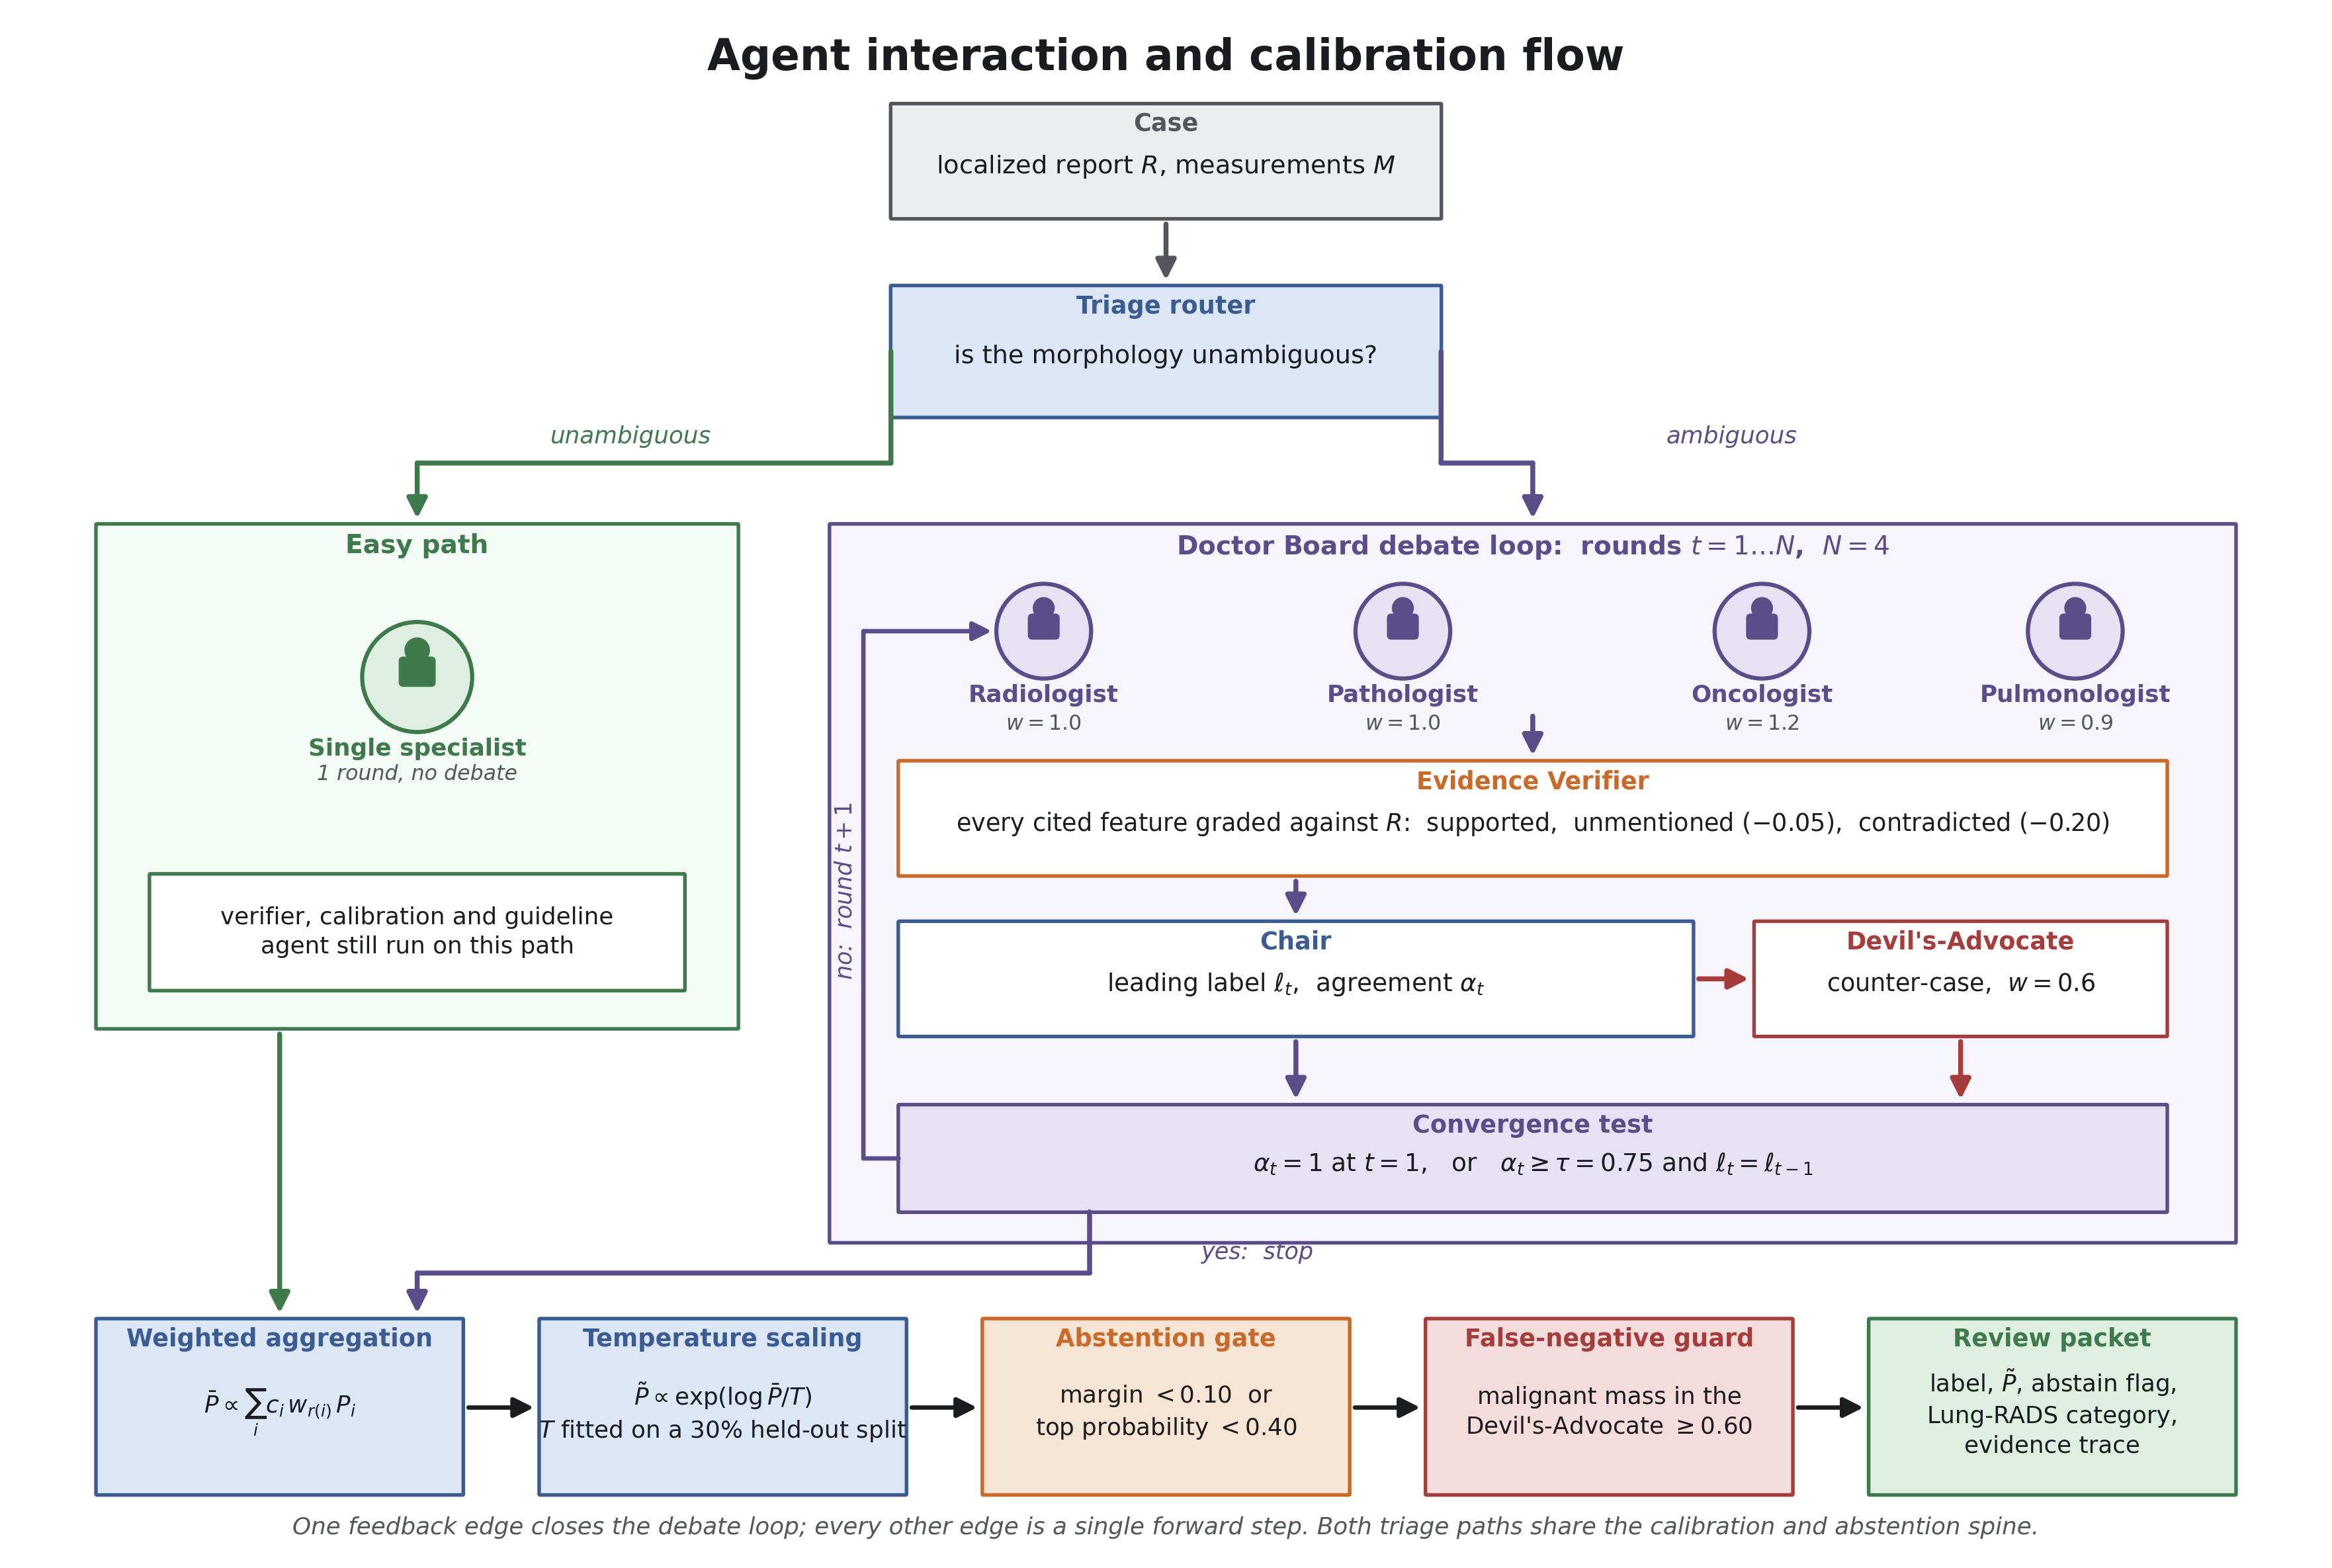
\includegraphics[width=0.98\textwidth]{figures/agent-flow.png}
\caption{Agent interaction and calibration flow.}
\label{fig:flow}
\end{figure*}

% ALGOBOX-START
\begin{center}
\small
\renewcommand{\arraystretch}{1.35}
\begin{tabular}{|p{0.94\linewidth}|}
\hline
\textbf{Input:} report $R$; measurements $M$; roles $\mathcal{S}$ with $|\mathcal{S}|=4$; round limit $N=4$; agreement threshold $\tau=0.75$; role weights $w$. \\
\textbf{Output:} label $\hat y$; calibrated $\tilde P$; abstain flag $a$; guideline category $g$; evidence trace $E$; rounds used $t^{*}$. \\
1.\quad \textbf{begin} \\
2.\quad \hspace*{1.5em}$\ell_0 \gets \varnothing$;\quad $E \gets \varnothing$;\quad $t^{*} \gets N$ \\
3.\quad \hspace*{1.5em}\textbf{for} $t \gets 1$ \textbf{to} $N$ \textbf{do} \\
4.\quad \hspace*{3em}\textbf{for each} $s_i \in \mathcal{S}$ \textbf{do} \\
5.\quad \hspace*{4.5em}$(P_i, c_i, X_i) \gets s_i(R, M)$\quad // from report, not oracle \\
6.\quad \hspace*{4.5em}$(E, c_i) \gets \textsc{Verify}(X_i, R, E, c_i)$\quad // $-0.20$ hard, $-0.05$ soft \\
7.\quad \hspace*{3em}\textbf{end for} \\
8.\quad \hspace*{3em}$\ell_t \gets \arg\max_k \bar P_t(k)$;\quad $\alpha_t \gets$ \textsc{Agreement}$(\{P_i\})$ \\
9.\quad \hspace*{3em}$P_{\mathrm{dev}} \gets \textsc{DevilsAdvocate}(\ell_t, R, M)$ \\
10.\quad \hspace*{3em}\textbf{if} $(t = 1 \wedge \alpha_t = 1) \vee (\alpha_t \ge \tau \wedge \ell_t = \ell_{t-1})$ \textbf{then} \\
11.\quad \hspace*{4.5em}$t^{*} \gets t$;\quad \textbf{break} \\
12.\quad \hspace*{3em}\textbf{end if} \\
13.\quad \hspace*{1.5em}\textbf{end for} \\
14.\quad \hspace*{1.5em}$\bar P(k) \gets \sum_i c_i w_{r(i)} P_i(k) / \sum_i c_i w_{r(i)}$\quad // includes $P_{\mathrm{dev}}$ at $w=0.6$ \\
15.\quad \hspace*{1.5em}$(\hat y, \tilde P, a) \gets \textsc{CalibrateAndAbstain}(\bar P, \alpha_{t^{*}}, P_{\mathrm{dev}})$\quad // Algorithm 2 \\
16.\quad \hspace*{1.5em}$g \gets \textsc{LungRADS}(M, X)$ \\
17.\quad \hspace*{1.5em}\textbf{return} $(\hat y, \tilde P, a, g, E, t^{*})$ \\
18.\quad \textbf{end} \\
\hline
\end{tabular}
\end{center}
\vspace{-2pt}
\begin{center}
\small\textbf{Algorithm 1:} Doctor Board debate procedure.
\end{center}
\vspace{4pt}
% ALGOBOX-END

% ALGOBOX-START
\begin{center}
\small
\renewcommand{\arraystretch}{1.35}
\begin{tabular}{|p{0.94\linewidth}|}
\hline
\textbf{Input:} aggregate $\bar P$; agreement $\alpha$; Devil's-Advocate distribution $P_{\mathrm{dev}}$; fitted temperature $T$ from the held-out split; margin $\delta=0.10$; floor $\phi=0.40$; guard $\gamma=0.60$. \\
\textbf{Output:} label $\hat y$; calibrated $\tilde P$; abstain flag $a$. \\
1.\quad \textbf{begin} \\
2.\quad \hspace*{1.5em}$\tilde P(k) \gets \exp(\log \bar P(k)/T) / \sum_j \exp(\log \bar P(j)/T)$\quad $\forall k$ \\
3.\quad \hspace*{1.5em}$(\tilde p_1, \tilde p_2, \tilde p_3) \gets \textsc{Sort}(\tilde P)$\quad // descending \\
4.\quad \hspace*{1.5em}$\hat y \gets \arg\max_k \tilde P(k)$;\quad $a \gets \textsc{false}$ \\
5.\quad \hspace*{1.5em}\textbf{if} $(\tilde p_1 - \tilde p_2) < \delta \vee \tilde p_1 < \phi$ \textbf{then} \\
6.\quad \hspace*{3em}$a \gets \textsc{true}$\quad // low margin or low confidence \\
7.\quad \hspace*{1.5em}\textbf{end if} \\
8.\quad \hspace*{1.5em}\textbf{if} $\hat y = \textsc{pre-invasive} \wedge P_{\mathrm{dev}}(\textsc{min.inv}) + P_{\mathrm{dev}}(\textsc{inv}) \ge \gamma$ \textbf{then} \\
9.\quad \hspace*{3em}$a \gets \textsc{true}$\quad // false-negative guard \\
10.\quad \hspace*{1.5em}\textbf{end if} \\
11.\quad \hspace*{1.5em}\textbf{return} $(\hat y, \tilde P, a)$ \\
12.\quad \textbf{end} \\
\hline
\end{tabular}
\end{center}
\vspace{-2pt}
\begin{center}
\small\textbf{Algorithm 2:} Calibration and abstention procedure.
\end{center}
\vspace{4pt}
% ALGOBOX-END

\subsection{Resource-use design}\label{sec:resource}

Three design choices bound the computation a case consumes, and each is measured rather than asserted. First, the triage router sends cases with unambiguous morphology to a single specialist and one round, reserving the four-role board for cases that need deliberation; Section~4.6 reports the resulting calls per case together with the under-triage rate that bounds how far this can safely be pushed. Second, the Chair's convergence test stops the debate as soon as a super-majority is stable across two rounds, so the round budget is an upper bound rather than a fixed cost. Third, that budget is itself capped at four rounds, which bounds the worst case. The accounting unit throughout is the language-model call, counted by an instrumented backend that wraps every detector, judge, specialist, critique, and summary call. For a pipeline whose work is dominated by model inference, the call count is the quantity that drives latency, price, and energy draw [35], which is why it is reported alongside the safety metrics rather than as an afterthought.


Direct hardware profiling is deliberately out of scope at this stage. Because the reasoning backbone is a deterministic mock backend rather than a served model, wall-clock latency, processor and accelerator utilization, and memory footprint measured on this harness would characterize the harness and not a deployment. Those quantities become meaningful once a real vision-language model is substituted at the documented interface, and we treat them as the first measurements to add at that point, with the call count serving as the hardware-independent proxy until then.

\subsection{Stress regimes}

A clean synthetic distribution cannot exercise safety machinery: there are no unsupported claims, borderline lesions, or distribution shift to catch. We therefore define five regimes over one generator, and a \emph{perceived}-versus-\emph{oracle} split in which the report and the specialists see the perceived features while all scoring uses the oracle. \textbf{Clean:} perceived $=$ oracle; balanced classes. \textbf{Noisy:} each perceived categorical or boolean feature is corrupted with probability $0.25$ and the report omits a truly-present sign with probability $0.30$. \textbf{Borderline:} only cases whose top-two malignancy posteriors lie within $0.20$ are retained. \textbf{Imbalanced:} the class prior is skewed toward pre-invasive ($0.60/0.25/0.15$). \textbf{Adversarial:} noise, borderline sampling, and a degraded detector (wider mask scatter, more misses) combined.

\subsection{Metrics}

Over answered (non-abstained) cases we report accuracy and macro-F1; over all cases, accuracy counting abstentions as wrong, and answer coverage. \textbf{Safety.} The false-negative rate is the fraction of truly-malignant nodules (minimally-invasive or invasive) answered as pre-invasive. AURC is the area under the risk--coverage curve over answered cases ranked by confidence (lower is better). Abstention value is $\mathrm{err}(\text{abstained})-\mathrm{err}(\text{answered})$; a positive value means the gate withholds the harder cases. \textbf{Calibration.} ECE with 10 equal-width bins, computed for the raw aggregate ($T{=}1$) and for the fitted-temperature output, together with the fitted $T$. \textbf{Grounding.} Verifier hard-flag precision and recall against the oracle, where the recall denominator is agent \emph{fabrications} only (claims that disagree with both the oracle and the perceived input), so that perception error, which is outside the verifier's scope, is not counted against it. \textbf{Cost.} Mean language-model calls per case (every detector, judge, specialist, critique, and summary call is counted through an instrumented backend) and the under-triage rate: cases the router sends down the easy path that are genuinely ambiguous by the oracle.

\subsection{Reproducible configuration}\label{sec:config}

A criticism of the original description is that the parameters that govern its behaviour (the DBSCAN neighbourhood and minimum count, the number of detection experts and judges, the number of agents and debate rounds, the convergence rule, and any calibration) are not stated. Every such value here lives in a single configuration object and is reported. The Nodule Spotter uses five detection experts and a three-member judging panel; masks are clustered with DBSCAN at $\varepsilon = 0.5$ (equivalently an IoU threshold of 0.5) and a minimum of two masks, and each cluster is averaged and binarized at 0.5. Hard cases use the four roles listed above with a maximum of four debate rounds and a convergence threshold of $\tau = 0.75$; easy cases use a single role and one round. The abstention gate uses a top-1/top-2 margin threshold of $0.10$, a top-probability floor of $0.40$, and a Devil's-Advocate guard threshold of $0.60$ on malignant probability mass. The calibration temperature is not fixed: it is fitted per run (Section~3.3). Changing any value and re-running propagates through the whole harness, which is what makes the ablation and the regime sweep controlled comparisons rather than anecdotes.

\subsection{Experimental design}

Each regime uses n=64 generated cases per seed across 8 seeds; 30\% of each run is held out to fit the calibration temperature and the remaining 70\% is scored, with the same split taken for every ablation variant so all are evaluated on identical test cases. We report the seed mean and standard deviation, and, where a claim rests on a comparison, a paired bootstrap over the shared case pool (1000 resamples) giving the effect size, its 95\% interval, and a two-sided p-value. The leave-one-component-out ablation disables one mechanism at a time. The mock backend is a deterministic function of the seed, so every number in this paper reproduces exactly; the accompanying test suite covers the regime generators, the report-grounded verifier, the temperature fitting, the safety gates, the call accounting, and the bootstrap.

\section{Results}\label{sec:results}
\subsection{Full system across regimes}
\begin{table}[htbp]
\centering
\small
\renewcommand{\arraystretch}{1.25}
\setlength{\tabcolsep}{5pt}
\begin{adjustbox}{max width=\linewidth}
\begin{tabular}{|l|c|c|c|c|c|c|c|}
\hline
\rowcolor{tblhead}
\textbf{Regime} & \textbf{acc(all)} & \textbf{acc(ans)} & \textbf{macro-F1} & \textbf{coverage} & \textbf{FNR} & \textbf{AURC} & \textbf{calls/case} \\ \hline
clean & $0.822\,{\pm}\,0.052$ & $0.920\,{\pm}\,0.053$ & $0.715\,{\pm}\,0.186$ & $0.894\,{\pm}\,0.043$ & $0.003\,{\pm}\,0.008$ & $0.015\,{\pm}\,0.012$ & $10.84\,{\pm}\,0.27$ \\
\hline
noisy & $0.789\,{\pm}\,0.069$ & $0.866\,{\pm}\,0.060$ & $0.573\,{\pm}\,0.148$ & $0.911\,{\pm}\,0.044$ & $0.010\,{\pm}\,0.012$ & $0.066\,{\pm}\,0.035$ & $10.84\,{\pm}\,0.39$ \\
\hline
borderline & $0.447\,{\pm}\,0.098$ & $0.633\,{\pm}\,0.075$ & $0.549\,{\pm}\,0.097$ & $0.714\,{\pm}\,0.157$ & $0.019\,{\pm}\,0.040$ & $0.350\,{\pm}\,0.066$ & $12.84\,{\pm}\,0.39$ \\
\hline
imbalanced & $0.497\,{\pm}\,0.072$ & $0.693\,{\pm}\,0.076$ & $0.676\,{\pm}\,0.085$ & $0.717\,{\pm}\,0.067$ & $0.000\,{\pm}\,0.000$ & $0.153\,{\pm}\,0.050$ & $12.04\,{\pm}\,0.61$ \\
\hline
adversarial & $0.197\,{\pm}\,0.071$ & $0.302\,{\pm}\,0.098$ & $0.243\,{\pm}\,0.089$ & $0.650\,{\pm}\,0.061$ & $0.051\,{\pm}\,0.042$ & $0.688\,{\pm}\,0.093$ & $11.41\,{\pm}\,0.22$ \\
\hline
\end{tabular}
\end{adjustbox}
\caption{Full-system results by regime.}
\label{tab:main}
\end{table}


Table~2 reports the full system across all five regimes as the seed mean and standard deviation; accuracy and coverage fall and AURC rises as the regime hardens, since the instrumentation is built to track the degradation rather than conceal it. On clean data the full system answers 0.894 of cases at 0.920 accuracy on answered cases, with a false-negative rate of 0.003 and AURC 0.015. Feature noise costs a few points of accuracy; borderline sampling and class imbalance roughly halve accuracy over all cases, mostly through increased abstention (coverage 0.71 and 0.72 respectively); and the adversarial regime drives accuracy over all cases to 0.197 and AURC to 0.688. Every metric moves in the direction a reviewer would predict, which is the purpose of the harness: the safety instrumentation should register stress, not mask it. Figure~3 shows accuracy and coverage together. Per-class counts are small at this $n$, which inflates macro-F1 variance; the accuracy, cost, calibration, and verifier results are the stable ones.


\begin{figure}[htbp]
\centering
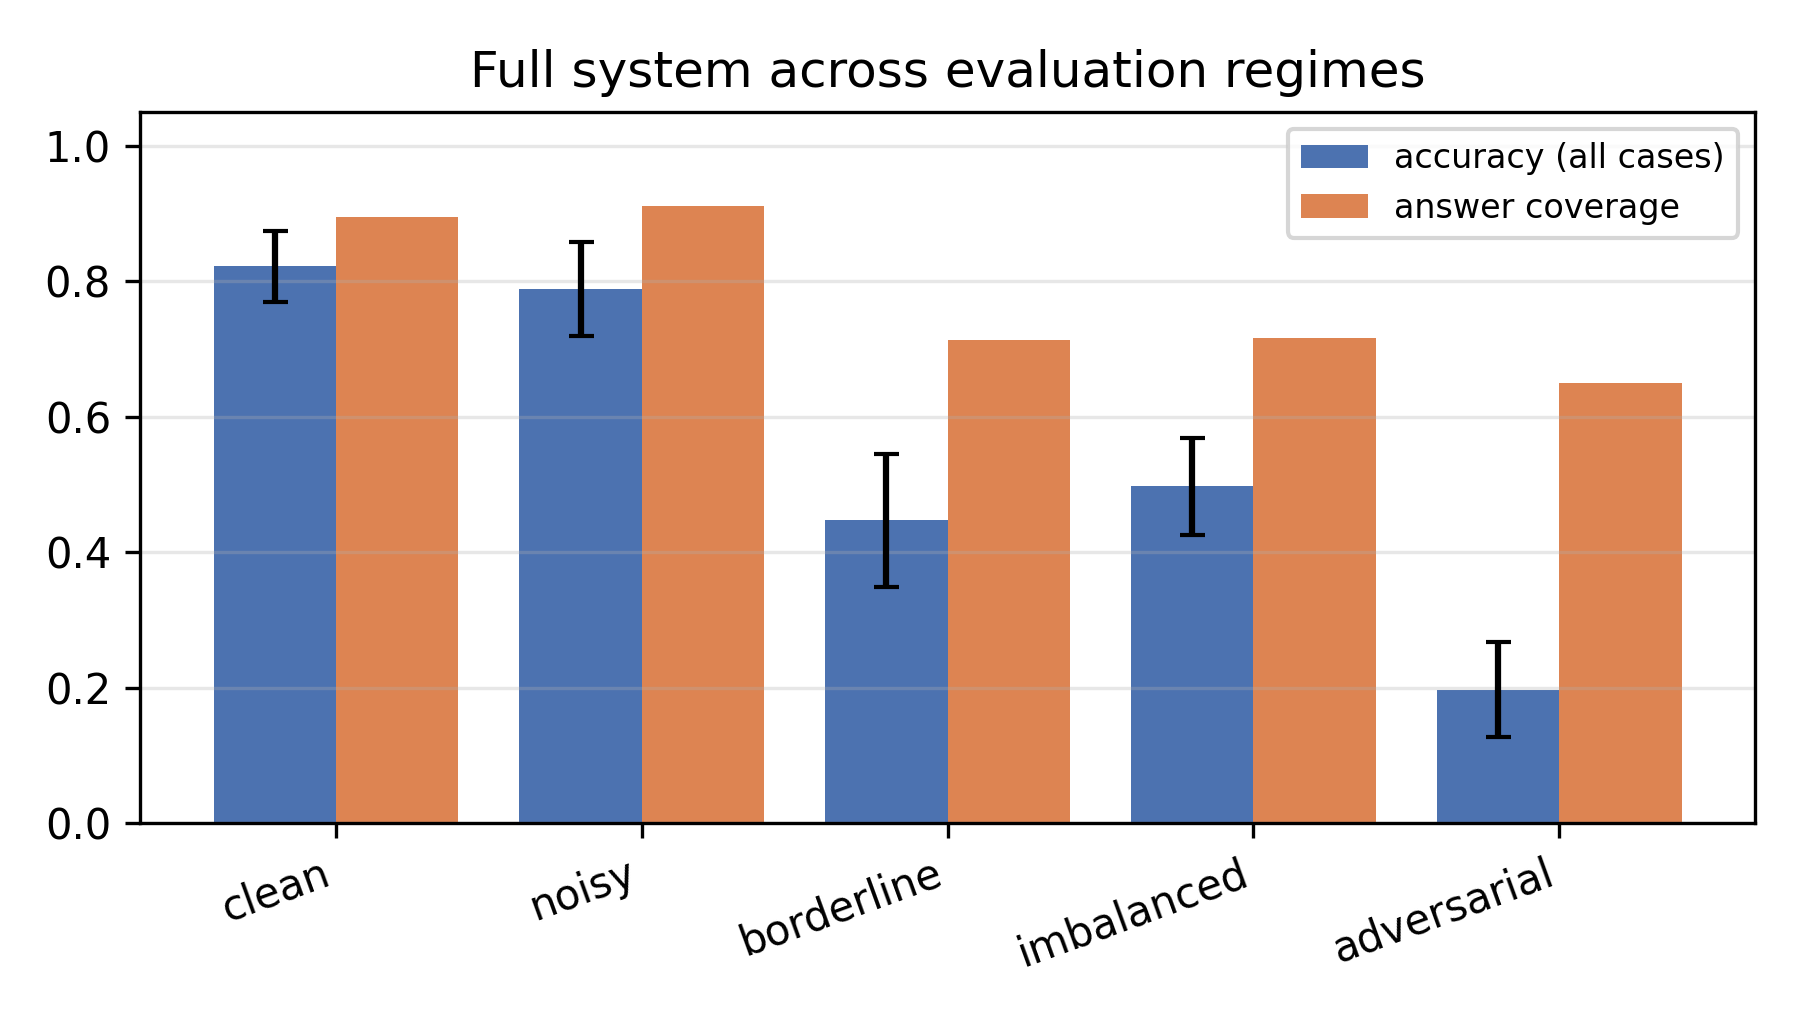
\includegraphics[width=0.86\textwidth]{figures/accuracy-by-regime.png}
\caption{Full-system accuracy and coverage by regime.}
\label{fig:acc}
\end{figure}

\subsection{Leave-one-component-out ablation}
\begin{table}[htbp]
\centering
\small
\renewcommand{\arraystretch}{1.25}
\setlength{\tabcolsep}{5pt}
\begin{adjustbox}{max width=\linewidth}
\begin{tabular}{|l|c|c|c|c|c|c|c|}
\hline
\rowcolor{tblhead}
\textbf{variant} & \textbf{acc(all)} & \textbf{macro-F1} & \textbf{cover} & \textbf{FNR} & \textbf{AURC} & \textbf{ECE} & \textbf{calls} \\ \hline
full & 0.822 & 0.715 & 0.894 & 0.003 & 0.015 & 0.108 & 10.8 \\
\hline
- router & 0.822 & 0.708 & 0.897 & 0.003 & 0.016 & 0.107 & 11.2 \\
\hline
- verifier & 0.822 & 0.715 & 0.894 & 0.003 & 0.015 & 0.105 & 10.8 \\
\hline
- devils\_advocate & 0.894 & 0.765 & 0.997 & 0.035 & 0.020 & 0.106 & 8.6 \\
\hline
- guideline & 0.822 & 0.715 & 0.894 & 0.003 & 0.015 & 0.108 & 10.8 \\
\hline
- calibration & 0.819 & 0.723 & 0.886 & 0.003 & 0.014 & 0.105 & 10.8 \\
\hline
- abstention & 0.903 & 0.780 & 1.000 & 0.026 & 0.020 & 0.112 & 10.8 \\
\hline
- board (1 agent) & 0.800 & 0.686 & 0.903 & 0.010 & 0.020 & 0.103 & 7.1 \\
\hline
- debate (1 round) & 0.803 & 0.714 & 0.883 & 0.003 & 0.013 & 0.092 & 9.8 \\
\hline
\end{tabular}
\end{adjustbox}
\caption{Ablation under the clean regime.}
\label{tab:abl-clean}
\end{table}

\begin{table}[htbp]
\centering
\small
\renewcommand{\arraystretch}{1.25}
\setlength{\tabcolsep}{5pt}
\begin{adjustbox}{max width=\linewidth}
\begin{tabular}{|l|c|c|c|c|c|c|c|}
\hline
\rowcolor{tblhead}
\textbf{variant} & \textbf{acc(all)} & \textbf{macro-F1} & \textbf{cover} & \textbf{FNR} & \textbf{AURC} & \textbf{ECE} & \textbf{calls} \\ \hline
full & 0.447 & 0.549 & 0.714 & 0.019 & 0.350 & 0.166 & 12.8 \\
\hline
- router & 0.450 & 0.542 & 0.725 & 0.019 & 0.363 & 0.168 & 13.2 \\
\hline
- verifier & 0.447 & 0.548 & 0.717 & 0.019 & 0.344 & 0.164 & 12.8 \\
\hline
- devils\_advocate & 0.542 & 0.568 & 0.900 & 0.082 & 0.350 & 0.132 & 10.3 \\
\hline
- guideline & 0.447 & 0.549 & 0.714 & 0.019 & 0.350 & 0.166 & 12.8 \\
\hline
- calibration & 0.478 & 0.515 & 0.794 & 0.019 & 0.355 & 0.166 & 12.8 \\
\hline
- abstention & 0.581 & 0.545 & 1.000 & 0.113 & 0.360 & 0.136 & 12.8 \\
\hline
- board (1 agent) & 0.286 & 0.552 & 0.467 & 0.043 & 0.323 & 0.134 & 7.1 \\
\hline
- debate (1 round) & 0.358 & 0.588 & 0.547 & 0.011 & 0.337 & 0.201 & 9.9 \\
\hline
\end{tabular}
\end{adjustbox}
\caption{Ablation under the borderline regime.}
\label{tab:abl-borderline}
\end{table}

\begin{table}[htbp]
\centering
\small
\renewcommand{\arraystretch}{1.25}
\setlength{\tabcolsep}{5pt}
\begin{adjustbox}{max width=\linewidth}
\begin{tabular}{|l|c|c|c|c|c|c|c|}
\hline
\rowcolor{tblhead}
\textbf{variant} & \textbf{acc(all)} & \textbf{macro-F1} & \textbf{cover} & \textbf{FNR} & \textbf{AURC} & \textbf{ECE} & \textbf{calls} \\ \hline
full & 0.197 & 0.243 & 0.650 & 0.051 & 0.688 & 0.217 & 11.4 \\
\hline
- router & 0.200 & 0.234 & 0.678 & 0.062 & 0.689 & 0.231 & 11.9 \\
\hline
- verifier & 0.194 & 0.239 & 0.650 & 0.051 & 0.690 & 0.218 & 11.4 \\
\hline
- devils\_advocate & 0.258 & 0.282 & 0.783 & 0.093 & 0.680 & 0.201 & 9.1 \\
\hline
- guideline & 0.197 & 0.243 & 0.650 & 0.051 & 0.688 & 0.217 & 11.4 \\
\hline
- calibration & 0.264 & 0.263 & 0.861 & 0.062 & 0.683 & 0.479 & 11.4 \\
\hline
- abstention & 0.344 & 0.322 & 1.000 & 0.132 & 0.679 & 0.157 & 11.4 \\
\hline
- board (1 agent) & 0.128 & 0.206 & 0.453 & 0.042 & 0.681 & 0.236 & 7.1 \\
\hline
- debate (1 round) & 0.172 & 0.257 & 0.539 & 0.047 & 0.683 & 0.216 & 9.8 \\
\hline
\end{tabular}
\end{adjustbox}
\caption{Ablation under the adversarial regime.}
\label{tab:abl-adversarial}
\end{table}


Tables~3, 4, and 5 report the ablation under the clean, borderline, and adversarial regimes respectively. The role-differentiated board is the dominant contributor to accuracy in four of five regimes: reducing it to a single agent lowers accuracy over all cases by up to 0.161 (borderline) and raises both AURC and ECE. The exception is the imbalanced regime, where the single agent scores 0.064 higher on accuracy over all cases ($p=0.006$): under a benign-heavy prior the board's role biases (the oncologist over-weights malignancy) and a fixed abstention margin combine to withhold or over-call cases a single unbiased radiologist would answer. Role weights and abstention thresholds are therefore deployment parameters that must be tuned to the target prevalence, not architecture constants; the harness surfaces this rather than averaging it away. Removing the router leaves accuracy essentially unchanged but raises cost (Section~4.6). Removing the verifier or the guideline agent does not move aggregate accuracy (their endpoints are grounding, reported in Section~4.4, and auditability, confirmed by the guideline agent's unit tests), while removing the Devil's-Advocate or the abstention gate trades coverage for false-negative rate (Section~4.3). Figure~4 visualizes the adversarial-regime ablation, where the dashed line marks the full system; because the confidence signal is uninformative under this regime, AURC barely moves while accuracy and false-negative rate still separate the components.


\begin{figure*}[htbp]
\centering
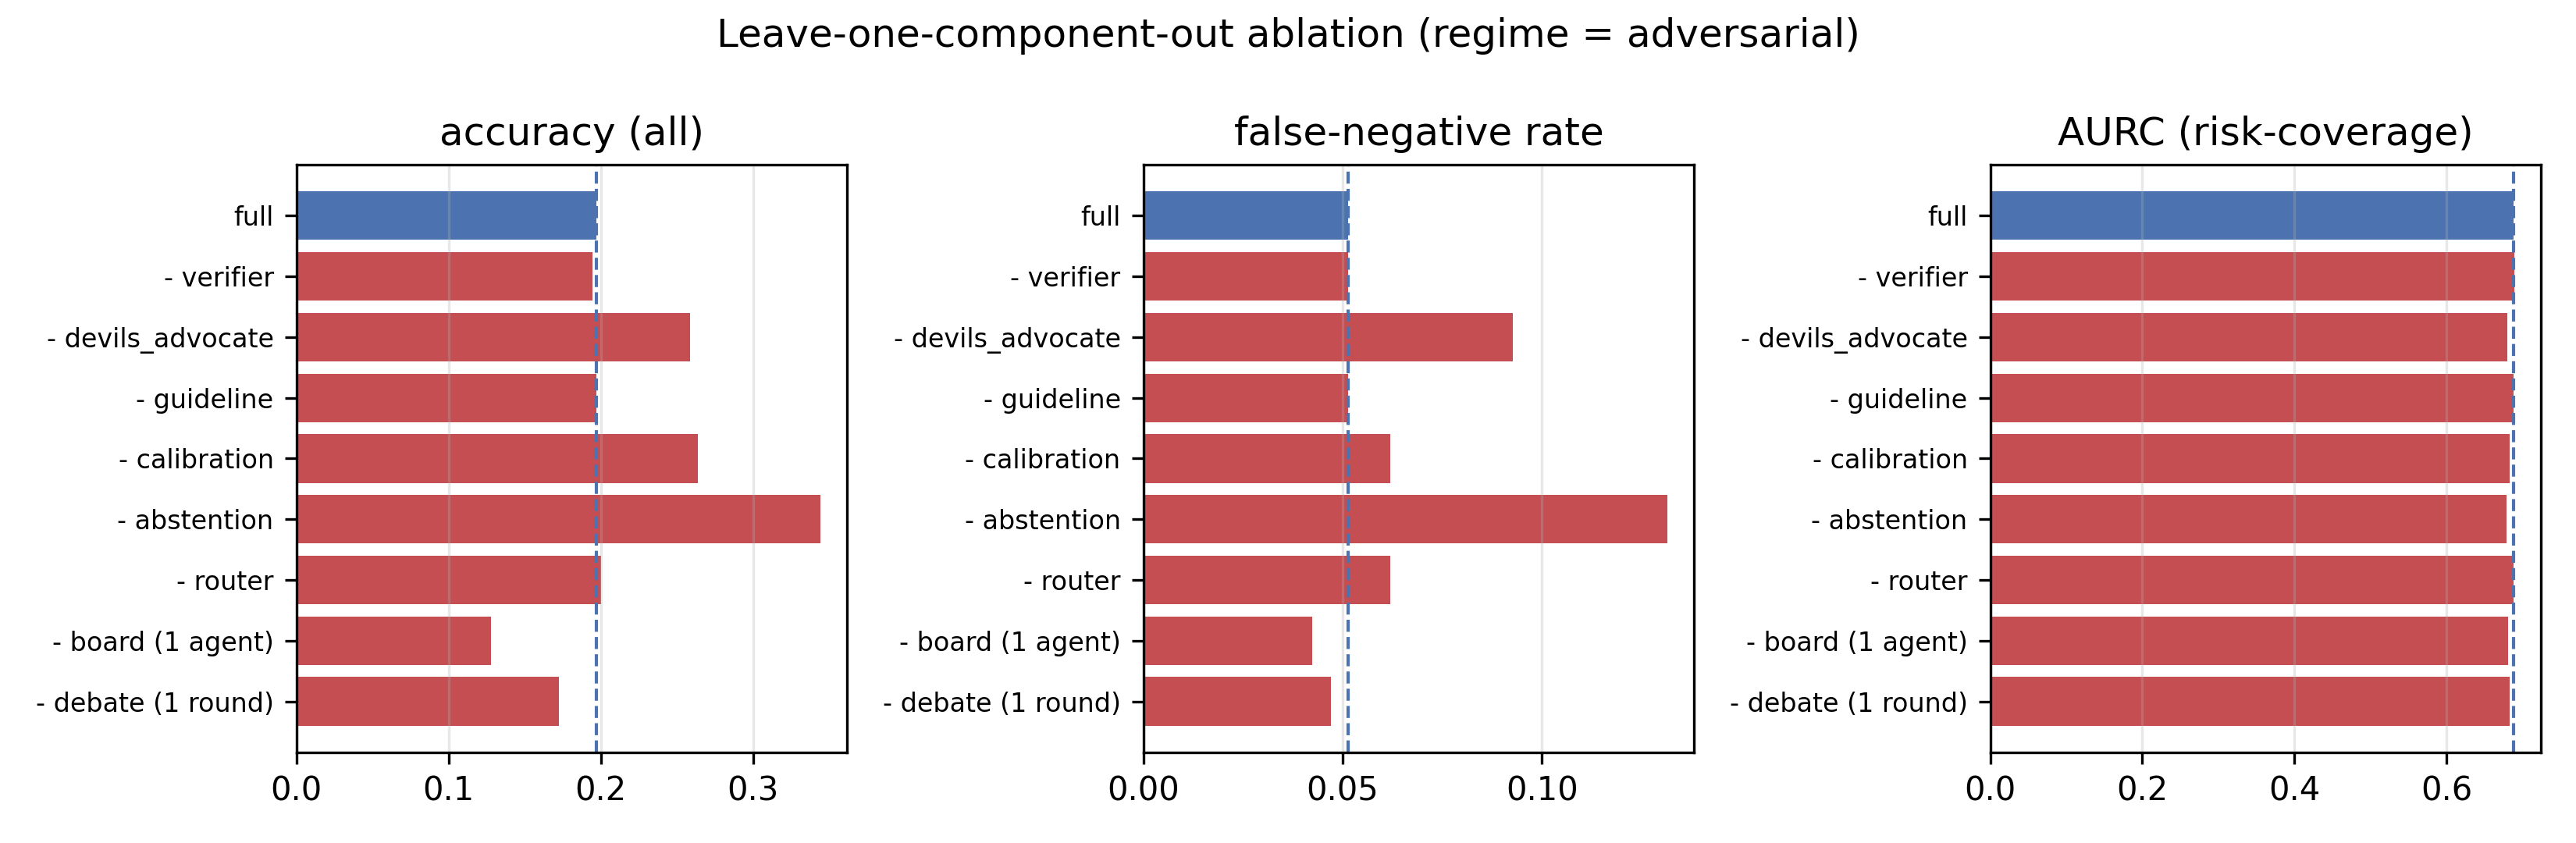
\includegraphics[width=0.98\textwidth]{figures/ablation-adversarial.png}
\caption{Leave-one-component-out ablation under the adversarial regime.}
\label{fig:abl}
\end{figure*}

\subsection{Abstention and the false-negative guard}\label{sec:abst}
\begin{table}[htbp]
\centering
\small
\renewcommand{\arraystretch}{1.25}
\setlength{\tabcolsep}{5pt}
\begin{adjustbox}{max width=\linewidth}
\begin{tabular}{|l|c|c|c|c|c|}
\hline
\rowcolor{tblhead}
\textbf{Regime} & \textbf{coverage} & \textbf{abst.\ value} & \textbf{abst.\ prec.} & \textbf{FNR (full)} & \textbf{FNR ($-$devil)} \\ \hline
clean & 0.894 & 0.125 & 0.205 & 0.003 & 0.035 \\
\hline
noisy & 0.911 & 0.360 & 0.494 & 0.010 & 0.051 \\
\hline
borderline & 0.714 & 0.173 & 0.540 & 0.019 & 0.082 \\
\hline
imbalanced & 0.717 & -0.242 & 0.065 & 0.000 & 0.006 \\
\hline
adversarial & 0.650 & -0.112 & 0.585 & 0.051 & 0.093 \\
\hline
\end{tabular}
\end{adjustbox}
\caption{Abstention and the false-negative guard, by regime.}
\label{tab:abst}
\end{table}


Table~6 reports abstention value, precision, and false-negative rate by regime, where abstention value is $\mathrm{err}_{\mathrm{abst}}-\mathrm{err}_{\mathrm{ans}}$ and is positive when the gate withholds the harder cases. The margin-based abstention gate has clearly positive value under the clean (0.125), noisy (0.360), and borderline (0.173) regimes: the withheld cases are markedly more error-prone than the answered ones. It is negative under class imbalance (-0.242, with abstention precision only 0.065) and under the adversarial regime (-0.112): a benign-heavy prior or heavy perception noise breaks the correlation between the aggregate's margin and its correctness, so a small margin no longer signals a likely error. This is a genuine negative result (selective prediction is only as good as the confidence signal it reads [33]), and it argues for pairing the confidence gate with a structural safeguard. The Devil's-Advocate false-negative guard is such a safeguard: it escalates whenever the board leans benign while a credible malignant counter-case exists, and it lowers the false-negative rate wherever false negatives occur (borderline 0.082$\to$0.019, $p<0.001$; adversarial 0.093$\to$0.051, $p=0.002$) at a coverage cost.

\subsection{Evidence verifier}\label{sec:ver}
\begin{table}[htbp]
\centering
\small
\renewcommand{\arraystretch}{1.25}
\setlength{\tabcolsep}{5pt}
\begin{adjustbox}{max width=\linewidth}
\begin{tabular}{|l|c|c|c|}
\hline
\rowcolor{tblhead}
\textbf{Regime} & \textbf{flag precision} & \textbf{flag recall} & \textbf{hard flags/case} \\ \hline
clean & $1.00\,{\pm}\,0.00$ & $1.00\,{\pm}\,0.00$ & $0.69\,{\pm}\,0.07$ \\
\hline
noisy & $0.90\,{\pm}\,0.06$ & $1.00\,{\pm}\,0.00$ & $0.53\,{\pm}\,0.03$ \\
\hline
borderline & $0.99\,{\pm}\,0.03$ & $1.00\,{\pm}\,0.00$ & $0.96\,{\pm}\,0.10$ \\
\hline
imbalanced & $1.00\,{\pm}\,0.00$ & $1.00\,{\pm}\,0.00$ & $0.89\,{\pm}\,0.12$ \\
\hline
adversarial & $0.89\,{\pm}\,0.05$ & $1.00\,{\pm}\,0.00$ & $0.59\,{\pm}\,0.08$ \\
\hline
\end{tabular}
\end{adjustbox}
\caption{Evidence verifier precision, recall, and flag rate by regime.}
\label{tab:verifier}
\end{table}


Table~7 reports flag precision, recall, and mean hard flags per case by regime. The verifier flags every agent-fabricated citation (recall 1.00 across all regimes) because the check against a parsed report is deterministic. Precision against the oracle is 1.00 on clean data and 0.89 under the adversarial regime, where a corrupted report occasionally leads the verifier to hard-flag a claim that happens to match the oracle. The verifier's scope is explicit and reported: it catches inconsistency between an agent and the shared report, not error already baked into the report by perception. Figure~5 plots precision and recall with the mean number of hard flags raised per case.


\begin{figure}[htbp]
\centering
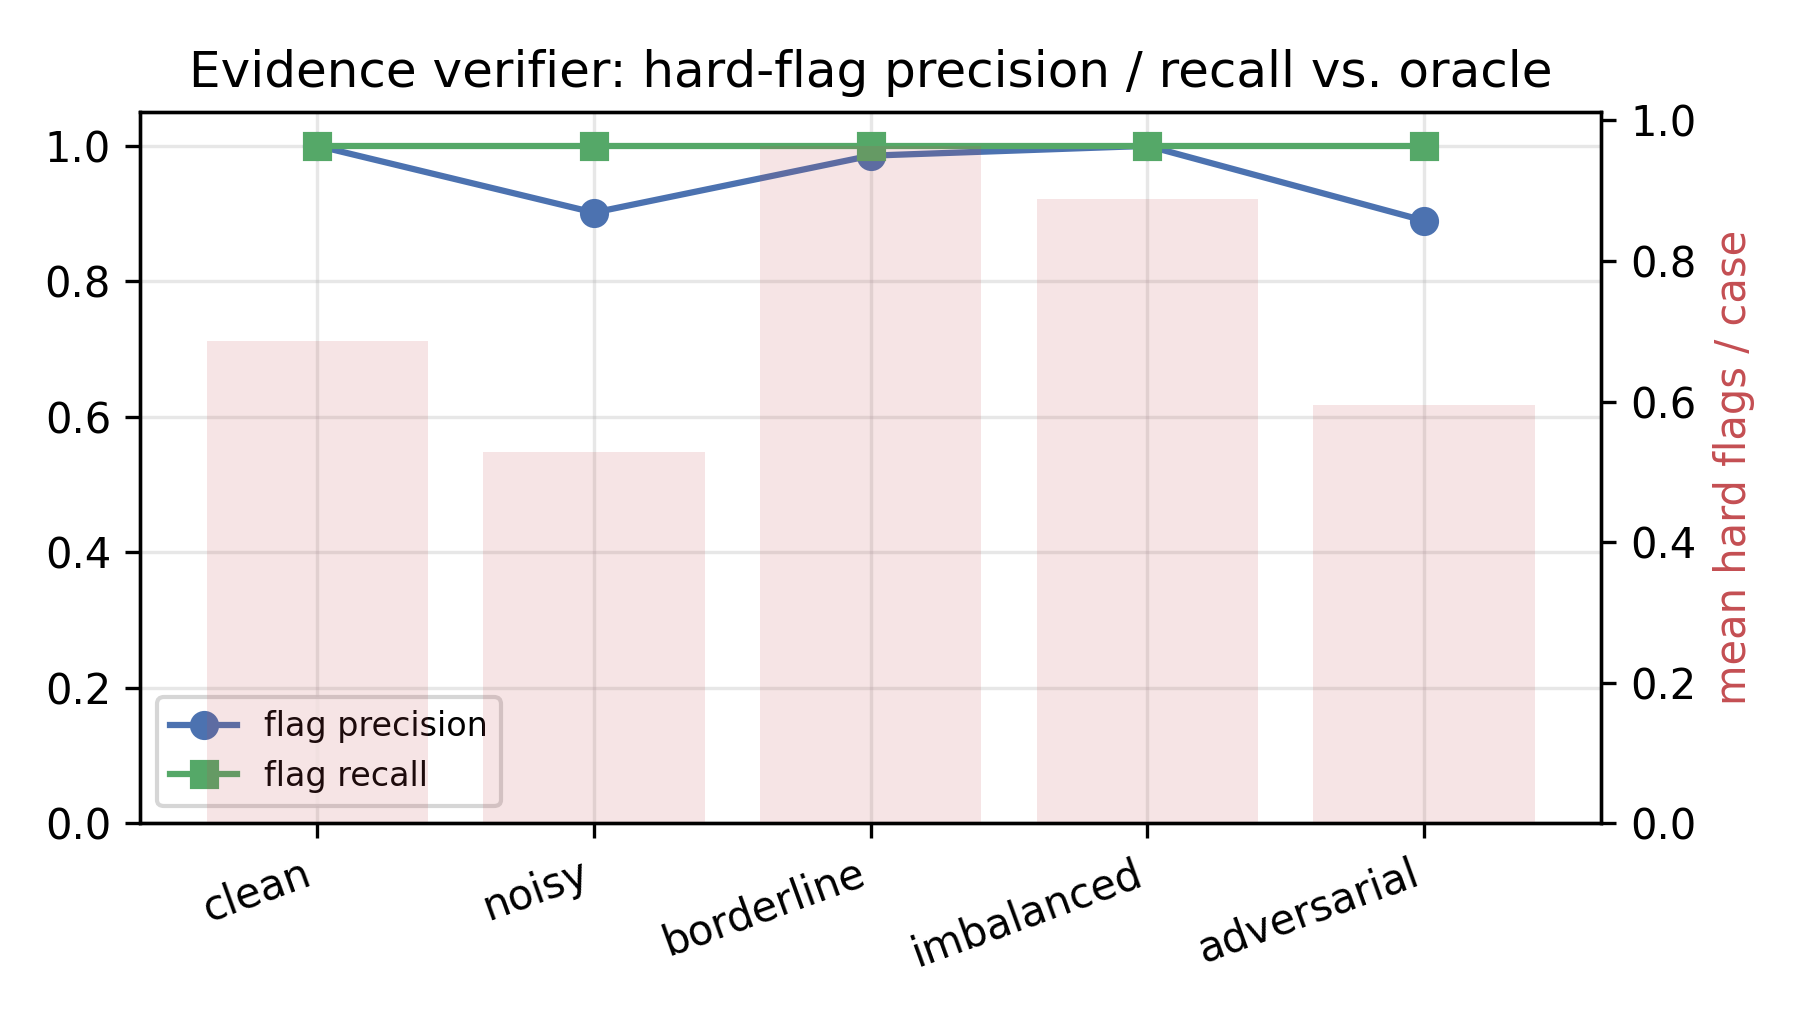
\includegraphics[width=0.86\textwidth]{figures/verifier-pr.png}
\caption{Verifier precision, recall, and hard-flag rate by regime.}
\label{fig:verifier}
\end{figure}

\subsection{Calibration}
\begin{table}[htbp]
\centering
\small
\renewcommand{\arraystretch}{1.25}
\setlength{\tabcolsep}{5pt}
\begin{adjustbox}{max width=\linewidth}
\begin{tabular}{|l|c|c|c|c|}
\hline
\rowcolor{tblhead}
\textbf{Regime} & \textbf{ECE ($T{=}1$)} & \textbf{ECE (fitted $T$)} & \textbf{fitted $T$} & \textbf{mean conf $-$ acc} \\ \hline
clean & $0.109\,{\pm}\,0.030$ & $0.108\,{\pm}\,0.037$ & $0.66\,{\pm}\,0.29$ & $-0.004\,{\pm}\,0.088$ \\
\hline
noisy & $0.086\,{\pm}\,0.035$ & $0.118\,{\pm}\,0.040$ & $1.10\,{\pm}\,0.39$ & $-0.034\,{\pm}\,0.086$ \\
\hline
borderline & $0.155\,{\pm}\,0.043$ & $0.166\,{\pm}\,0.039$ & $1.79\,{\pm}\,0.97$ & $-0.023\,{\pm}\,0.122$ \\
\hline
imbalanced & $0.125\,{\pm}\,0.014$ & $0.157\,{\pm}\,0.067$ & $0.81\,{\pm}\,0.31$ & $0.101\,{\pm}\,0.105$ \\
\hline
adversarial & $0.540\,{\pm}\,0.101$ & $0.217\,{\pm}\,0.086$ & $3.96\,{\pm}\,0.12$ & $0.201\,{\pm}\,0.101$ \\
\hline
\end{tabular}
\end{adjustbox}
\caption{Calibration error and fitted temperature by regime.}
\label{tab:calib}
\end{table}


Table~8 reports calibration error and the fitted temperature by regime; the temperature is fitted by NLL minimization on a 30\% held-out split, and it spans well below and well above 1, so no single fixed value serves all regimes. On clean data the aggregate is already close to calibrated (ECE 0.109) and the fitted temperature is 0.66, a mild sharpening. Under the adversarial regime the raw aggregate is badly overconfident (ECE 0.540; mean confidence exceeds accuracy by 0.201), the fitted temperature rises to 3.96, and ECE falls to 0.217 (paired $\Delta$ -0.262, $p<0.001$). In the other four regimes the fitted temperature stays near 1 and the change in ECE is not significant. Temperature scaling is thus a no-op when the model is already calibrated and a large, significant correction exactly when distribution shift makes it overconfident [31]; it should be fitted on a small labelled calibration set drawn from the deployment distribution, not hard-coded. Figure~6 shows ECE before and after scaling.


\begin{figure}[htbp]
\centering
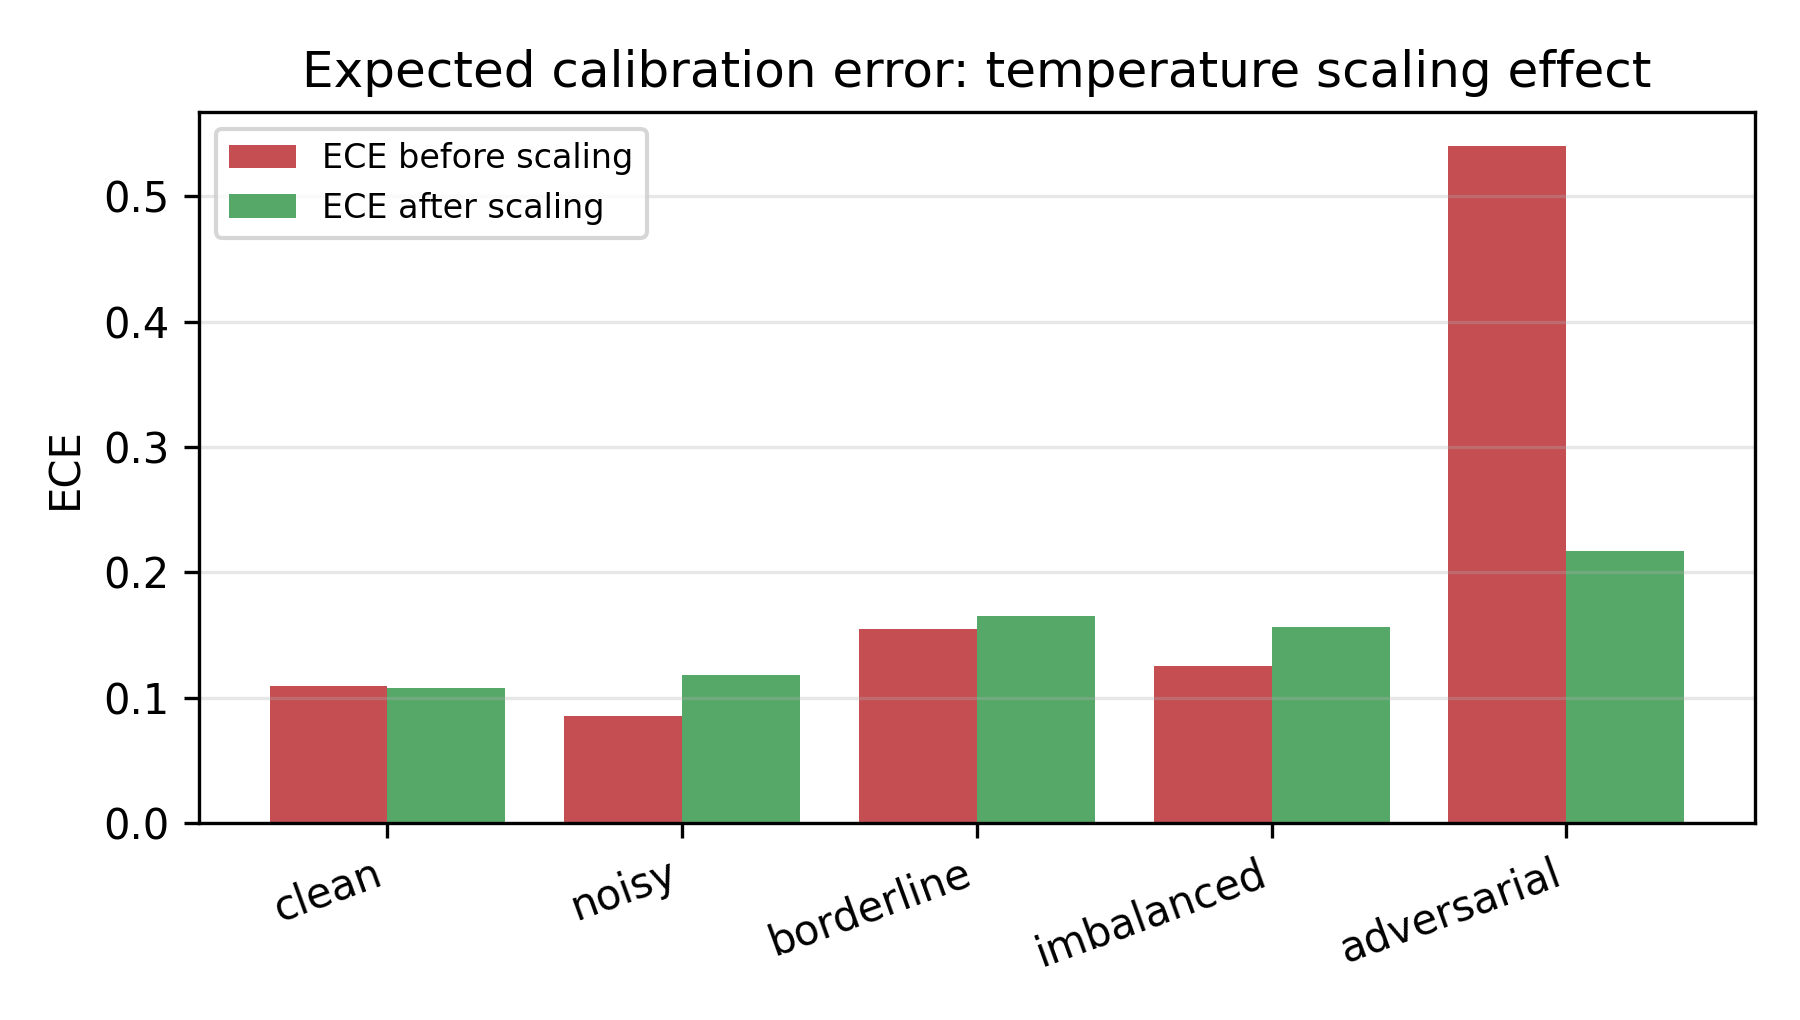
\includegraphics[width=0.86\textwidth]{figures/calibration-ece.png}
\caption{Calibration error before and after temperature scaling.}
\label{fig:calib}
\end{figure}

\subsection{Cost of adaptive routing}\label{sec:cost}
\begin{table}[htbp]
\centering
\small
\renewcommand{\arraystretch}{1.25}
\setlength{\tabcolsep}{5pt}
\begin{adjustbox}{max width=\linewidth}
\begin{tabular}{|l|c|c|c|c|c|}
\hline
\rowcolor{tblhead}
\textbf{Regime} & \textbf{calls: always board} & \textbf{calls: adaptive} & \textbf{frac.\ easy} & \textbf{under-triage} & \textbf{$\Delta$ calls [95\% CI]} \\ \hline
clean & 11.16 & 10.84 & 0.10 & 0.014 & $-0.31$ [$-0.42$, $-0.22$] \\
\hline
noisy & 11.19 & 10.84 & 0.10 & 0.044 & $-0.35$ [$-0.49$, $-0.22$] \\
\hline
borderline & 13.16 & 12.84 & 0.06 & 0.022 & $-0.31$ [$-0.48$, $-0.18$] \\
\hline
imbalanced & 12.47 & 12.04 & 0.11 & 0.022 & $-0.43$ [$-0.58$, $-0.30$] \\
\hline
adversarial & 11.89 & 11.41 & 0.10 & 0.086 & $-0.48$ [$-0.66$, $-0.31$] \\
\hline
\end{tabular}
\end{adjustbox}
\caption{Cost of adaptive routing by regime.}
\label{tab:cost}
\end{table}


Table~9 reports calls per case, routed-easy fraction, and under-triage rate by regime, with a negative $\Delta$ meaning the router is cheaper. Adaptive routing lowers mean calls per case in every regime (clean 11.16$\to$10.84, $p<0.001$), but the effect is small in absolute terms: on this distribution only 6--11\% of cases have morphology unambiguous enough to route easy, and the remainder legitimately reach the full board. The realizable saving is bounded below by the single-agent cost ($\approx$7.1 calls/case, from the \texttt{-\,board} ablation) and scales with that easy fraction, a distribution-dependent quantity that a deployment can measure and, if desired, widen by loosening the triage predicate. The under-triage rate (genuinely ambiguous cases sent down the easy path) rises from 0.014 on clean data to 0.086 under the adversarial regime, quantifying the router's failure mode: perception noise makes some hard cases look easy, so a deployment should bias the router toward escalation when its inputs are noisy. The routing cost saving is significant in every regime ($p<0.001$; Table~11). Figure~7 contrasts the two policies.


\begin{figure}[htbp]
\centering
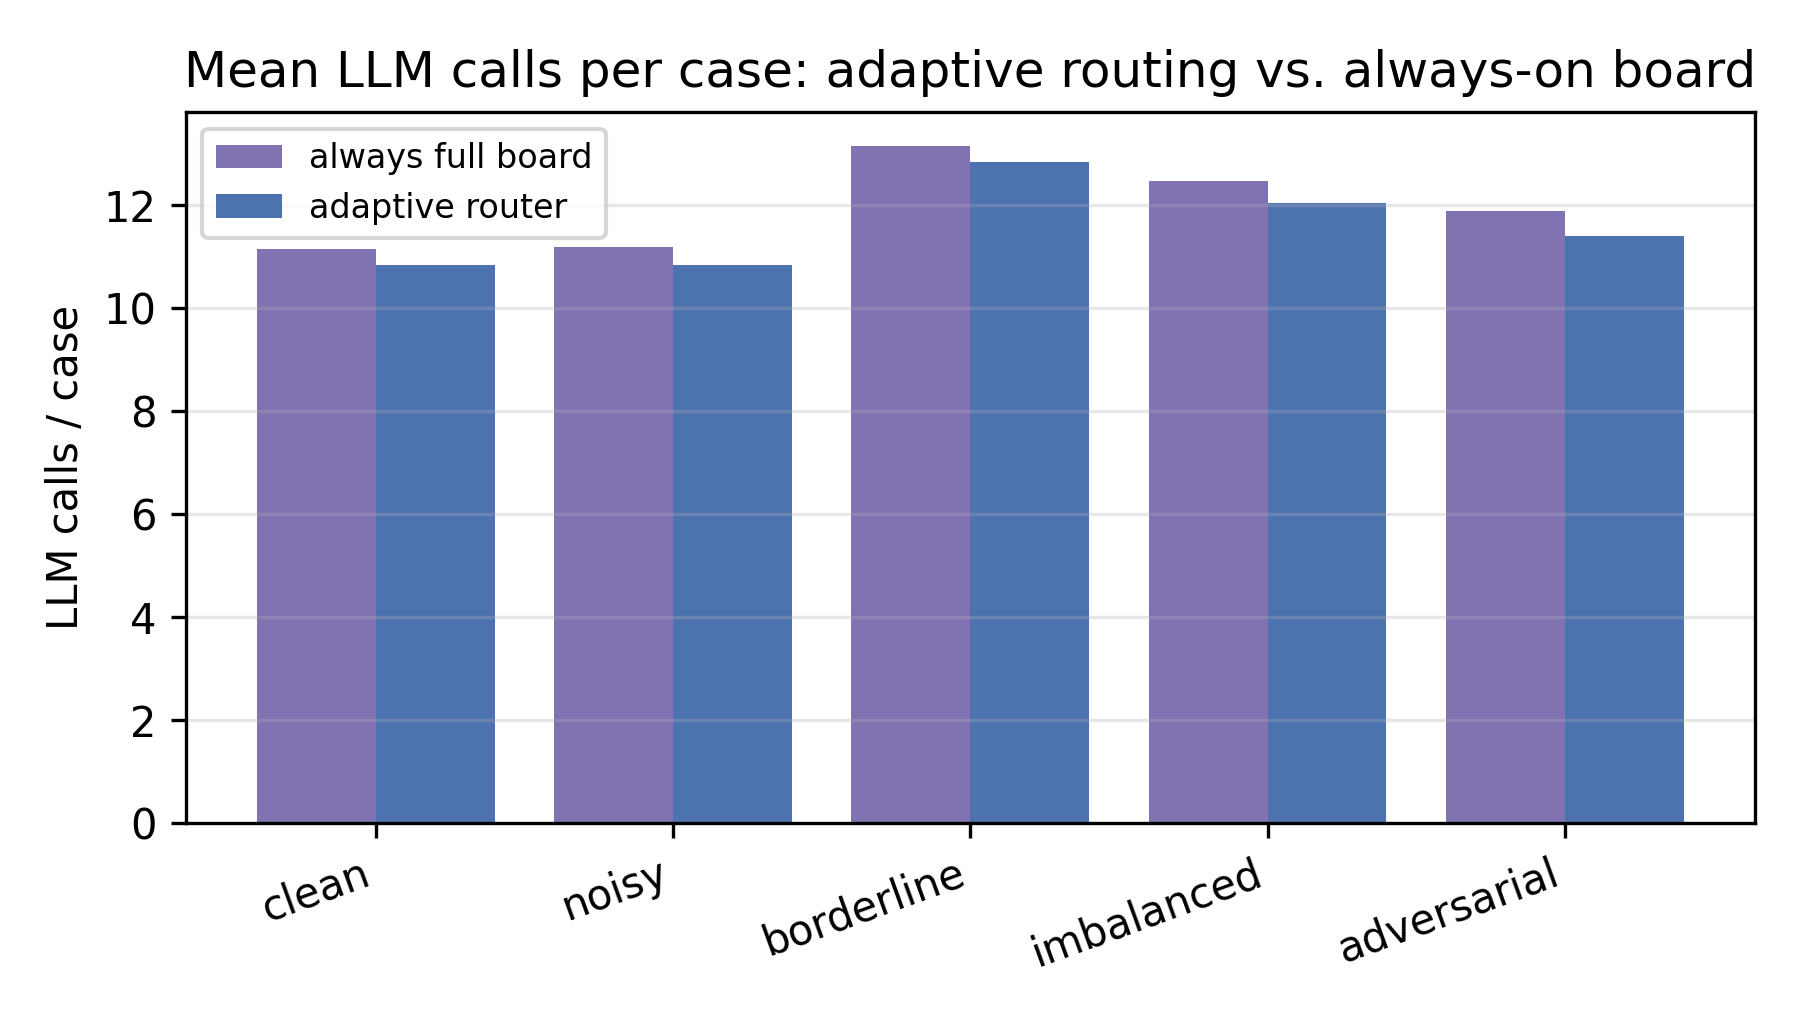
\includegraphics[width=0.86\textwidth]{figures/cost-routing.png}
\caption{Mean language-model calls per case by routing policy.}
\label{fig:cost}
\end{figure}

\begin{table}[htbp]
\centering
\small
\renewcommand{\arraystretch}{1.25}
\setlength{\tabcolsep}{5pt}
\begin{adjustbox}{max width=\linewidth}
\begin{tabular}{|l|c|c|c|c|}
\hline
\rowcolor{tblhead}
\textbf{Regime} & \textbf{tokens: always board} & \textbf{tokens: adaptive} & \textbf{tokens saved} & \textbf{calls saved} \\ \hline
clean & 2347 & 2234 & 4.8\% & 2.8\% \\
\hline
noisy & 2333 & 2209 & 5.3\% & 3.1\% \\
\hline
borderline & 2955 & 2848 & 3.6\% & 2.4\% \\
\hline
imbalanced & 2736 & 2585 & 5.5\% & 3.5\% \\
\hline
adversarial & 2568 & 2402 & 6.5\% & 4.0\% \\
\hline
\end{tabular}
\end{adjustbox}
\caption{Prompt and response volume per case by routing policy.}
\label{tab:tokens}
\end{table}


Call count is a coarse unit: the calls the router removes are the expensive ones. Table~10 meters the actual prompt and response volume per case, counted by the same instrumented backend and converted at four characters per token. Because a board call carries a role-specific knowledge excerpt and the full report while a triage call carries neither, the proportional saving in tokens exceeds the saving in calls in every regime, by a factor of between 1.5 and 1.7. This matters for the sustainability claim: inference energy and monetary cost both scale with the volume of text a served model processes rather than with the number of requests [35,40], so it is the token reduction, not the call reduction, that transfers to a deployment. The orchestration itself is negligible against that: the full pipeline, excluding model inference, runs in approximately seven milliseconds per case on a single commodity CPU core, against the hundreds of milliseconds a single served-model call typically costs, so the coordination the architecture adds is not a latency bottleneck.

\subsection{Significance summary}

Table~11 collects the paired bootstrap significance tests referenced throughout this section, summarizing which effects are significant in which regime.

\begin{table}[htbp]
\centering
\small
\renewcommand{\arraystretch}{1.25}
\setlength{\tabcolsep}{5pt}
\begin{adjustbox}{max width=\linewidth}
\begin{tabular}{|l|l|c|c|r|}
\hline
\rowcolor{tblhead}
\textbf{Regime} & \textbf{comparison} & \textbf{$\Delta$} & \textbf{95\% CI} & \textbf{p} \\ \hline
clean & board vs.\ single agent (acc all) & $+0.022$ & [$-0.008$, $+0.050$] & 0.172 \\
\hline
clean & adaptive vs.\ always board (calls/case) & $-0.314$ & [$-0.417$, $-0.219$] & 0.000 \\
\hline
clean & fitted vs.\ no calibration (ECE) & $+0.002$ & [$-0.055$, $+0.019$] & 0.368 \\
\hline
clean & with vs.\ without Devil's-Advocate (FNR) & $-0.032$ & [$-0.051$, $-0.013$] & 0.000 \\
\hline
noisy & board vs.\ single agent (acc all) & $+0.064$ & [$+0.031$, $+0.094$] & 0.000 \\
\hline
noisy & adaptive vs.\ always board (calls/case) & $-0.347$ & [$-0.495$, $-0.217$] & 0.000 \\
\hline
noisy & fitted vs.\ no calibration (ECE) & $+0.032$ & [$-0.017$, $+0.040$] & 0.372 \\
\hline
noisy & with vs.\ without Devil's-Advocate (FNR) & $-0.041$ & [$-0.066$, $-0.022$] & 0.000 \\
\hline
borderline & board vs.\ single agent (acc all) & $+0.161$ & [$+0.114$, $+0.214$] & 0.000 \\
\hline
borderline & adaptive vs.\ always board (calls/case) & $-0.314$ & [$-0.475$, $-0.181$] & 0.000 \\
\hline
borderline & fitted vs.\ no calibration (ECE) & $+0.000$ & [$-0.057$, $+0.071$] & 0.994 \\
\hline
borderline & with vs.\ without Devil's-Advocate (FNR) & $-0.063$ & [$-0.095$, $-0.032$] & 0.000 \\
\hline
imbalanced & board vs.\ single agent (acc all) & $-0.064$ & [$-0.108$, $-0.019$] & 0.006 \\
\hline
imbalanced & adaptive vs.\ always board (calls/case) & $-0.431$ & [$-0.583$, $-0.297$] & 0.000 \\
\hline
imbalanced & fitted vs.\ no calibration (ECE) & $+0.033$ & [$-0.027$, $+0.059$] & 0.294 \\
\hline
imbalanced & with vs.\ without Devil's-Advocate (FNR) & $-0.006$ & [$-0.024$, $+0.000$] & 0.772 \\
\hline
adversarial & board vs.\ single agent (acc all) & $+0.069$ & [$+0.042$, $+0.100$] & 0.000 \\
\hline
adversarial & adaptive vs.\ always board (calls/case) & $-0.481$ & [$-0.661$, $-0.311$] & 0.000 \\
\hline
adversarial & fitted vs.\ no calibration (ECE) & $-0.262$ & [$-0.305$, $-0.243$] & 0.000 \\
\hline
adversarial & with vs.\ without Devil's-Advocate (FNR) & $-0.041$ & [$-0.073$, $-0.015$] & 0.002 \\
\hline
\end{tabular}
\end{adjustbox}
\caption{Paired bootstrap significance tests by regime and comparison.}
\label{tab:sig}
\end{table}

\subsection{Qualitative case trace}

The pipeline emits a review packet per case. For a representative adversarial-regime case the trace reads: detection IoU $0.76$; report \enquote{a ground-glass density nodule with an irregular shape and lobulated margin \ldots there is spiculation}; router decision \emph{hard} (part-solid-like, mid-size); four specialists opine, the verifier hard-flags one pathologist citation of \texttt{cavitation} as contradicted by the report; the Devil's-Advocate argues pre-invasive; the Chair records a super-majority for invasive at round~2; calibration with the fitted $T$ yields $\tilde P = (0.02,\,0.15,\,0.83)$; the guideline agent returns \emph{Lung-RADS~4X} driven by spiculation and documented interval growth. The label, the calibrated probabilities, the flagged claim, the dissent, and the guideline category together form what a qualified reader would inspect; the system is decision support, not an autonomous diagnosis.

\section{Discussion}\label{sec:disc}
\subsection{Safety and cost as measurable properties}

The value of the enhancement is that each mechanism has an endpoint and a number. The board earns its cost through accuracy and macro-F1 where ambiguity exists. The router earns its complexity through a significant if modest reduction in calls, with a named and quantified failure mode. The verifier earns its place through complete fabrication recall and an explicitly bounded scope. Fitted calibration earns its place by removing calibration error where the model is overconfident and doing nothing where it is not. The abstention gate is reported honestly, including the two regimes in which it is counter-productive. This is the opposite of an \enquote{always be definitive} policy: the system is permitted, and measured, to say less. We regard the reporting of negative results (the imbalanced-regime board reversal, the loss of abstention value under shift) as part of the contribution, because a harness that only ever confirms its own design is not a safety evaluation.


Read together, the measured reduction in computational overhead and the measured improvement in calibration are what a sustainability argument for multi-agent clinical AI has to rest on [36,37]: not a claim that more agents are better, but evidence that the extra deliberation is spent only where it changes the answer, and that the confidence attached to that answer can be trusted. The saving demonstrated here is modest in absolute terms, two to four percent of calls per case, and it is bounded below by the single-agent cost; what the harness contributes is the accounting discipline that makes a saving of this kind visible, attributable, and auditable at all.

\subsection{When confidence-based abstention fails}

The clearest lesson is Section~4.3: selective prediction depends on the confidence signal being informative, and under class imbalance and the adversarial regime it is not [15,33]. Two responses follow. First, abstention value should be monitored in deployment; a non-positive value is a signal that the confidence signal has degraded and that the thresholds should not be trusted. Second, the confidence gate should be paired with structural checks that do not read a calibrated probability at all, such as the Devil's-Advocate false-negative guard, which lowers the false-negative rate even when the aggregate's confidence is uninformative.

\subsection{Prevalence sensitivity of the board}

The imbalanced-regime reversal is worth stating plainly: role weighting that helps on a balanced distribution can hurt when the base rate shifts. The oncologist's malignancy bias and a fixed abstention margin, tuned implicitly for balanced classes, together push accuracy over all cases below that of a single unbiased radiologist. Role weights and abstention thresholds are therefore deployment parameters that should be re-fitted to the target prevalence alongside the calibration temperature, and the value of a multi-agent board should be re-checked on the operating distribution rather than assumed from a balanced benchmark.

\subsection{Comparison with prior multi-agent medical systems}

MedAgents [23], MDAgents [24], and MedAgent-Pro [25] demonstrate that role-structured collaboration and evidence-oriented workflows improve medical reasoning; MDAgents also adapts structure to difficulty. Our contribution is orthogonal: we take one such pipeline and make its safety and cost behaviour \emph{measurable}, with per-component endpoints, stress regimes, and paired significance tests, and we report where the mechanisms do not help. The verifier's report-grounding differs from self-consistency checks [34] in anchoring on the pipeline's own artefact, which keeps its scope inspectable.

\subsection{Threats to validity}

The evaluation is synthetic. The mock backend reasons from the same feature heuristic that generates the labels, so absolute accuracy is not meaningful and inter-agent error correlation is understated; the comparative, cost, calibration, and grounding results are the transferable ones. The verifier's report parser is a transparent rule set rather than a learned extractor. The guideline agent implements a subset of Lung-RADS v2022. The knowledge base is a short reference document. The detector is a perturbation model, not a trained network [6]. Per-class counts are small at this $n$, which widens macro-F1 intervals. Each of these is a single documented interface with a swap-in point; the experimental protocol (stress regimes, per-component endpoints, multi-seed intervals, paired tests) is what carries over to a real evaluation.

\subsection{Toward a clinical evaluation}

Replacing the synthetic generator with a LIDC-IDRI / DICOM loader [30], the mock backend with an image-grounded VLM [12,17], and the perturbation detector with a trained segmenter [6] leaves the orchestration, the metrics, and the harness unchanged. The same tables would then be produced on patient-level splits with radiologist-adjudicated ground truth, and the calibration temperature, the role weights, and the abstention thresholds would be fitted on a held-out clinical calibration set. Prospective reader studies would measure whether the review packet (label, calibrated probabilities, verifier trace, recorded dissent, and guideline category) changes radiologist decisions and time-to-decision.

\subsection{Deployment and governance considerations}

Three practices follow from the design. The evidence trace should be presented to a qualified reader, not consumed autonomously: the label, the calibrated probabilities, the supporting observations, the flagged claims, the recorded dissent, the guideline category, and the abstention status form a review packet whose purpose is to make the machine's reasoning auditable, not to replace the reader. Audit logs should retain the model version, the full configuration, the random seed where applicable, the retrieved knowledge, and identifiers for every prompt and tool call, so that a surprising output can be reconstructed and investigated. And the safety endpoints reported here (abstention value, verifier flag rate, under-triage rate, calibration error) are exactly the quantities a post-market monitoring plan should track over time, because each of them can drift as scanners, protocols, and populations change, and a drop in abstention value in particular is an early signal that the confidence signal the gate depends on has degraded.

\section{Conclusion and Future Work}\label{sec:concl}

LungNoduleAgent-Enhanced keeps the detect--describe--diagnose pipeline of Yang et~al.~[27] and adds adaptive triage, a role-differentiated board, a report-grounded verifier, a Devil's-Advocate false-negative guard, guideline-grounded escalation, fitted temperature scaling, and margin-based abstention, each an instrumented component with an explicit success metric. Across five stress regimes with multi-seed intervals and paired significance tests, the board drives accuracy except under a benign-heavy prior, adaptive routing gives a small but significant and bounded cost reduction, the verifier achieves complete fabrication recall, and fitted calibration removes the calibration error that distribution shift introduces, while the abstention gate helps only where the confidence signal is informative.


The measured improvements are as follows. The role-differentiated board raises accuracy over all cases by up to 0.161 (borderline regime) against a single agent. Adaptive routing lowers mean language-model calls per case by two to four percent in every regime, significant at $p<0.001$ throughout, against a single-agent floor of $\approx$7.1 calls per case. Fitted temperature scaling cuts expected calibration error under the adversarial regime from 0.540 to 0.217, a relative reduction of 60\%, while leaving the already calibrated clean regime untouched. The evidence verifier reaches a fabrication recall of 1.00 across all regimes. The Devil's-Advocate guard lowers the false-negative rate from 0.082 to 0.019 under the borderline regime. Each figure is a seed mean over 8 seeds with paired significance testing.


Future work will (i)~replace the synthetic components with a trained detector, an image-grounded VLM, and LIDC-IDRI plus private cohorts; (ii)~fit role weights and abstention thresholds to the operating prevalence and re-run the harness; (iii)~add a disagreement-aware abstention rule and test it against the margin gate under shift; (iv)~run a prospective reader study on the review packet; and (v)~extend the cost accounting from call counts to measured energy and latency on served models, including deployment settings that matter for sustainable healthcare computing: edge inference close to the scanner, federated training across sites without moving patient data, and green AI scheduling that places deliberation-heavy cases on lower-carbon capacity [35,36,37]. The broader aim is a template for multi-agent clinical decision support in which safety, cost, and resource use are measured, not assumed.

\section*{Supplementary Materials}

The following checklist records what is needed to reproduce every number in this article. \textbf{Data.} No patient data are used. All cases are produced by the documented synthetic generator at 64 cases per seed across 8 seeds, so the dataset is regenerated exactly from a fixed seed rather than stored; the real-data path uses LIDC-IDRI [30] at the same documented interface. \textbf{Code.} The reference implementation, the deterministic mock language backend, the synthetic case generator, the evaluation harness, the figure and table scripts, and the automated test suite are released as a single repository at \url{https://github.com/LochanNarayan/SafeNodule-MAS}, and are also available from the corresponding author on request. \textbf{Configuration.} Every parameter is held in one configuration object and reported in Section~3.8: five detection experts, a three-member judging panel, DBSCAN at $\varepsilon=0.5$ with a minimum of two masks, four specialist roles, at most four debate rounds, a convergence threshold of $\tau=0.75$, an abstention margin of 0.10, a probability floor of 0.40, a Devil's-Advocate guard threshold of 0.60, and a 30\% calibration split. \textbf{Hardware.} No accelerator is required: the mock backend is a deterministic function of the seed, so the full protocol runs on a single commodity CPU, which is also why hardware-level energy and latency figures are deferred to the served-model setting (Section~3.5). \textbf{Randomness.} Every run is seeded; the reported values are seed means with standard deviations and paired bootstrap intervals over 1000 resamples.

\section*{Data Availability Statement}

Data available on request.

\section*{Conflicts of Interest}

The authors declare no conflicts of interest.

\begin{thebibliography}{99}
\small
\setlength{\bibsep}{2pt plus 1pt}
\bibitem{bray2024globocan}
Bray, F., Laversanne, M., Sung, H., Ferlay, J., Siegel, R. L., Soerjomataram, I., \& Jemal, A. (2024). Global cancer statistics 2022: GLOBOCAN estimates of incidence and mortality worldwide for 36 cancers in 185 countries. \textit{CA: A Cancer Journal for Clinicians, 74}(3), 229--263.

\bibitem{national2011nlst}
National Lung Screening Trial Research Team. (2011). Reduced lung-cancer mortality with low-dose computed tomographic screening. \textit{New England Journal of Medicine, 365}(5), 395--409.

\bibitem{macmahon2017fleischner}
MacMahon, H., Naidich, D. P., Goo, J. M., Lee, K. S., Leung, A. N. C., Mayo, J. R., \ldots\ Bankier, A. A. (2017). Guidelines for management of incidental pulmonary nodules detected on CT images: From the Fleischner Society 2017. \textit{Radiology, 284}(1), 228--243.

\bibitem{acr2022lungrads}
American College of Radiology. (2022). \textit{Lung CT Screening Reporting \& Data System (Lung-RADS) version 2022}. American College of Radiology, Reston, VA.

\bibitem{mcwilliams2013brock}
McWilliams, A., Tammemagi, M. C., Mayo, J. R., Roberts, H., Liu, G., Soghrati, K., \ldots\ Lam, S. (2013). Probability of cancer in pulmonary nodules detected on first screening CT. \textit{New England Journal of Medicine, 369}(10), 910--919.

\bibitem{isensee2021nnunet}
Isensee, F., Jaeger, P. F., Kohl, S. A. A., Petersen, J., \& Maier-Hein, K. H. (2021). nnU-Net: A self-configuring method for deep learning-based biomedical image segmentation. \textit{Nature Methods, 18}(2), 203--211.

\bibitem{achiam2023gpt4}
Achiam, J., Adler, S., Agarwal, S., Ahmad, L., Akkaya, I., Aleman, F. L., \ldots\ Zoph, B. (2023). GPT-4 technical report. \textit{arXiv preprint} arXiv:2303.08774.

\bibitem{anthropic2024claude}
Anthropic. (2024). \textit{The Claude 3 model family: Opus, Sonnet, Haiku} [Technical report]. Anthropic, San Francisco, CA.

\bibitem{bai2025qwen25vl}
Bai, S., Chen, K., Liu, X., Wang, J., Ge, W., Song, S., \ldots\ Lin, J. (2025). Qwen2.5-VL technical report. \textit{arXiv preprint} arXiv:2502.13923.

\bibitem{liu2023llava}
Liu, H., Li, C., Wu, Q., \& Lee, Y. J. (2023). Visual instruction tuning. In \textit{Advances in Neural Information Processing Systems} (Vol. 36, pp. 34892--34916).

\bibitem{li2023llavamed}
Li, C., Wong, C., Zhang, S., Usuyama, N., Liu, H., Yang, J., Naumann, T., Poon, H., \& Gao, J. (2023). LLaVA-Med: Training a large language-and-vision assistant for biomedicine in one day. \textit{arXiv preprint} arXiv:2306.00890.

\bibitem{sellergren2025medgemma}
Sellergren, A., Kazemzadeh, S., Jaroensri, R., Kiraly, A., Traverse, M., Kohlberger, T., \ldots\ Shetty, S. (2025). MedGemma technical report. \textit{arXiv preprint} arXiv:2507.05201.

\bibitem{lai2025medr1}
Lai, Y., Zhong, J., Li, M., Zhao, S., \& Yang, X. (2025). Med-R1: Reinforcement learning for generalizable medical reasoning in vision-language models. \textit{arXiv preprint} arXiv:2503.13939.

\bibitem{ji2023hallucination}
Ji, Z., Lee, N., Frieske, R., Yu, T., Su, D., Xu, Y., Ishii, E., Bang, Y. J., Madotto, A., \& Fung, P. (2023). Survey of hallucination in natural language generation. \textit{ACM Computing Surveys, 55}(12), 1--38.

\bibitem{xiong2024uncertainty}
Xiong, M., Hu, Z., Lu, X., Li, Y., Fu, J., He, J., \& Hooi, B. (2024). Can LLMs express their uncertainty? An empirical evaluation of confidence elicitation in LLMs. In \textit{International Conference on Learning Representations}.

\bibitem{singhal2023medpalm}
Singhal, K., Azizi, S., Tu, T., Mahdavi, S. S., Wei, J., Chung, H. W., \ldots\ Natarajan, V. (2023). Large language models encode clinical knowledge. \textit{Nature, 620}(7972), 172--180.

\bibitem{saab2024medgemini}
Saab, K., Tu, T., Weng, W.-H., Tanno, R., Stutz, D., Wulczyn, E., \ldots\ Natarajan, V. (2024). Capabilities of Gemini models in medicine. \textit{arXiv preprint} arXiv:2404.18416.

\bibitem{thirunavukarasu2023llmmedicine}
Thirunavukarasu, A. J., Ting, D. S. J., Elangovan, K., Gutierrez, L., Tan, T. F., \& Ting, D. S. W. (2023). Large language models in medicine. \textit{Nature Medicine, 29}(8), 1930--1940.

\bibitem{du2023debate}
Du, Y., Li, S., Torralba, A., Tenenbaum, J. B., \& Mordatch, I. (2024). Improving factuality and reasoning in language models through multiagent debate. In \textit{Proceedings of the 41st International Conference on Machine Learning} (pp. 11733--11763).

\bibitem{liang2023divergent}
Liang, T., He, Z., Jiao, W., Wang, X., Wang, Y., Wang, R., Yang, Y., Shi, S., \& Tu, Z. (2023). Encouraging divergent thinking in large language models through multi-agent debate. \textit{arXiv preprint} arXiv:2305.19118.

\bibitem{chan2023chateval}
Chan, C.-M., Chen, W., Su, Y., Yu, J., Xue, W., Zhang, S., Fu, J., \& Liu, Z. (2023). ChatEval: Towards better LLM-based evaluators through multi-agent debate. \textit{arXiv preprint} arXiv:2308.07201.

\bibitem{hong2024metagpt}
Hong, S., Zhuge, M., Chen, J., Zheng, X., Cheng, Y., Wang, J., \ldots\ Schmidhuber, J. (2024). MetaGPT: Meta programming for a multi-agent collaborative framework. In \textit{International Conference on Learning Representations}.

\bibitem{tang2023medagents}
Tang, X., Zou, A., Zhang, Z., Li, Z., Zhao, Y., Zhang, X., Cohan, A., \& Gerstein, M. (2023). MedAgents: Large language models as collaborators for zero-shot medical reasoning. \textit{arXiv preprint} arXiv:2311.10537.

\bibitem{kim2024mdagents}
Kim, Y., Park, C., Jeong, H., Chan, Y. S., Xu, X., McDuff, D., Lee, H., Ghassemi, M., Breazeal, C., \& Park, H. W. (2024). MDAgents: An adaptive collaboration of LLMs for medical decision-making. In \textit{Advances in Neural Information Processing Systems} (Vol. 37, pp. 79410--79452).

\bibitem{wang2025medagentpro}
Wang, Z., Wu, J., Cai, L., Low, C. H., Yang, X., Li, Q., \& Jin, Y. (2025). MedAgent-Pro: Towards evidence-based multi-modal medical diagnosis via reasoning agentic workflow. \textit{arXiv preprint} arXiv:2503.18968.

\bibitem{fallahpour2025medrax}
Fallahpour, A., Ma, J., Munim, A., Lyu, H., \& Wang, B. (2025). MedRAX: Medical reasoning agent for chest X-ray. \textit{arXiv preprint} arXiv:2502.02673.

\bibitem{yang2025lungnoduleagent}
Yang, C., Jin, H., Yu, X., Wang, Z., Liu, Y., Fan, F., Lei, D., Jia, G., Wang, C., \& Ge, R. (2025). LungNoduleAgent: A collaborative multi-agent system for precision diagnosis of lung nodules. \textit{arXiv preprint} arXiv:2511.21042.

\bibitem{xiao2025describe}
Xiao, X., Zhang, Y., Nguyen, T.-H., Lam, B.-T., Wang, J., Zhao, L., Hamm, J., Wang, T., Li, X., \& Wang, X. (2025). Describe anything in medical images. \textit{arXiv preprint} arXiv:2505.05804.

\bibitem{edge2024graphrag}
Edge, D., Trinh, H., Cheng, N., Bradley, J., Chao, A., Mody, A., Truitt, S., Metropolitansky, D., Ness, R. O., \& Larson, J. (2024). From local to global: A graph RAG approach to query-focused summarization. \textit{arXiv preprint} arXiv:2404.16130.

\bibitem{armato2011lidc}
Armato, S. G., III, McLennan, G., Bidaut, L., McNitt-Gray, M. F., Meyer, C. R., Reeves, A. P., \ldots\ Clarke, L. P. (2011). The Lung Image Database Consortium (LIDC) and Image Database Resource Initiative (IDRI): A completed reference database of lung nodules on CT scans. \textit{Medical Physics, 38}(2), 915--931.

\bibitem{guo2017calibration}
Guo, C., Pleiss, G., Sun, Y., \& Weinberger, K. Q. (2017). On calibration of modern neural networks. In \textit{Proceedings of the 34th International Conference on Machine Learning} (pp. 1321--1330).

\bibitem{naeini2015ece}
Naeini, M. P., Cooper, G. F., \& Hauskrecht, M. (2015). Obtaining well calibrated probabilities using Bayesian binning. In \textit{Proceedings of the AAAI Conference on Artificial Intelligence} (Vol. 29).

\bibitem{geifman2017selective}
Geifman, Y., \& El-Yaniv, R. (2017). Selective classification for deep neural networks. In \textit{Advances in Neural Information Processing Systems} (Vol. 30).

\bibitem{manakul2023selfcheckgpt}
Manakul, P., Liusie, A., \& Gales, M. J. F. (2023). SelfCheckGPT: Zero-resource black-box hallucination detection for generative large language models. In \textit{Proceedings of the 2023 Conference on Empirical Methods in Natural Language Processing} (pp. 9004--9017).

\bibitem{strubell2019energy}
Strubell, E., Ganesh, A., \& McCallum, A. (2019). Energy and policy considerations for deep learning in NLP. In \textit{Proceedings of the 57th Annual Meeting of the Association for Computational Linguistics} (pp. 3645--3650).

\bibitem{ueda2024climate}
Ueda, D., Walston, S. L., Fujita, S., Fushimi, Y., Tsuboyama, T., Kamagata, K., \ldots\ Naganawa, S. (2024). Climate change and artificial intelligence in healthcare: Review and recommendations towards a sustainable future. \textit{Diagnostic and Interventional Imaging, 105}(11), 453--459.

\bibitem{thomson2025environmental}
Thomson, R. M., Perdomo Lampignano, J., Fisher, E., Wati, C., Jeyakumar, G., Duncan, S., \& Lowe, D. J. (2025). Evaluating the environmental sustainability of AI in radiology: A systematic review of current practice. \textit{BMJ Digital Health and AI, 1}(1), e000073.

\bibitem{ester1996dbscan}
Ester, M., Kriegel, H.-P., Sander, J., \& Xu, X. (1996). A density-based algorithm for discovering clusters in large spatial databases with noise. In \textit{Proceedings of the 2nd International Conference on Knowledge Discovery and Data Mining (KDD)} (pp. 226--231).

\bibitem{kadavath2022knowwhat}
Kadavath, S., Conerly, T., Askell, A., Henighan, T., Drain, D., Perez, E., \ldots\ Kaplan, J. (2022). Language models (mostly) know what they know. \textit{arXiv preprint} arXiv:2207.05221.

\bibitem{luccioni2024power}
Luccioni, A. S., Jernite, Y., \& Strubell, E. (2024). Power hungry processing: Watts driving the cost of AI deployment? In \textit{Proceedings of the 2024 ACM Conference on Fairness, Accountability, and Transparency}.
\end{thebibliography}

\end{document}
